%% 
%% Copyright 2007-2024 Elsevier Ltd
%% 
%% This file is part of the 'Elsarticle Bundle'.
%% ---------------------------------------------
%% 
%% It may be distributed under the conditions of the LaTeX Project Public
%% License, either version 1.3 of this license or (at your option) any
%% later version.  The latest version of this license is in
%%    http://www.latex-project.org/lppl.txt
%% and version 1.3 or later is part of all distributions of LaTeX
%% version 1999/12/01 or later.
%% 
%% The list of all files belonging to the 'Elsarticle Bundle' is
%% given in the file `manifest.txt'.
%% 
%% Template article for Elsevier's document class `elsarticle'
%% with harvard style bibliographic references

%% \documentclass[preprint,12pt,authoryear]{elsarticle}

%% Use the option review to obtain double line spacing
%% \documentclass[authoryear,preprint,review,12pt]{elsarticle}

%% Use the options 1p,twocolumn; 3p; 3p,twocolumn; 5p; or 5p,twocolumn
%% for a journal layout:
\documentclass[final,1p,times,authoryear]{elsarticle}
%% \documentclass[final,1p,times,twocolumn,authoryear]{elsarticle}
%% \documentclass[final,3p,times,authoryear]{elsarticle}
%% \documentclass[final,3p,times,twocolumn,authoryear]{elsarticle}
%% \documentclass[final,5p,times,authoryear]{elsarticle}
%% \documentclass[final,5p,times,twocolumn,authoryear]{elsarticle}

%% For including figures, graphicx.sty has been loaded in
%% elsarticle.cls. If you prefer to use the old commands
%% please give \usepackage{epsfig}

%% The amssymb package provides various useful mathematical symbols
\usepackage{amssymb}
\usepackage{color}
%% The amsmath package provides various useful equation environments.
\usepackage{amsmath}
%% The amsthm package provides extended theorem environments
%% \usepackage{amsthm}

\usepackage{hyperref}
\usepackage{float}


%% The lineno packages adds line numbers. Start line numbering with
%% \begin{linenumbers}, end it with \end{linenumbers}. Or switch it on
%% for the whole article with \linenumbers.
%% \usepackage{lineno}
\usepackage{lmodern}
\usepackage{mdframed}
\usepackage{enumitem}
\usepackage{verbatim}
\usepackage{listings}
\usepackage{xcolor}

\lstnewenvironment{smalljson}
  {
    \scriptsize
    \lstset{
      basicstyle=\ttfamily,           % Typewriter font
      backgroundcolor=\color{gray!10}, % Light gray background
      frame=single,                   % Single frame around the code
      rulecolor=\color{black},        % Frame color
      breaklines=true,                % Break lines that are too long
      showstringspaces=false,         % Hide spaces in strings
      commentstyle=\color{green},     % Comment color
      keywordstyle=\color{blue},      % Keyword color
      stringstyle=\color{red},        % String color
      captionpos=b,                   % Caption position (bottom)
      escapeinside={\%*}{*)}          % To escape into LaTeX code
    }
  }
  {}

\journal{Digital Investigation}

\begin{document}

\begin{frontmatter}

%% Title, authors and addresses

%% use the tnoteref command within \title for footnotes;
%% use the tnotetext command for theassociated footnote;
%% use the fnref command within \author or \affiliation for footnotes;
%% use the fntext command for theassociated footnote;
%% use the corref command within \author for corresponding author footnotes;
%% use the cortext command for theassociated footnote;
%% use the ead command for the email address,
%% and the form \ead[url] for the home page:
%% \title{Title\tnoteref{label1}}
%% \tnotetext[label1]{}
%% \author{Name\corref{cor1}\fnref{label2}}
%% \ead{email address}
%% \ead[url]{home page}
%% \fntext[label2]{}
%% \cortext[cor1]{}
%% \affiliation{organization={},
%%            addressline={}, 
%%            city={},
%%            postcode={}, 
%%            state={},
%%            country={}}
%% \fntext[label3]{}

\title{Digital Forensic Readiness Model for 5G Core Networks} %% Article title

%% use optional labels to link authors explicitly to addresses:
%% \author[label1,label2]{}
%% \affiliation[label1]{organization={},
%%             addressline={},
%%             city={},
%%             postcode={},
%%             state={},
%%             country={}}
%%
%% \affiliation[label2]{organization={},
%%             addressline={},
%%             city={},
%%             postcode={},
%%             state={},
%%             country={}}

\author{Nathan Opperman\fnref{label1}}
\ead{u21553832@tuks.co.za}

\author{Sheunesu Makura\corref{cor1}\fnref{label2}}
\ead{makura.sm@up.ac.za}

% Affiliations
\author[label1,label2]{}
\affiliation{organization={DigiForS},
             addressline={University of Pretoria},
             city={Pretoria},
             postcode={0002},
             country={South Africa}}

%% Abstract
\begin{abstract}
The introduction of 5G technology represents a significant milestone for cellular network technology, with unprecedented speeds, reduced latency, better energy efficiency, and higher data rates. However, these advancements also introduce new challenges, particularly in cybersecurity and digital forensics. Traditional forensic methods, designed for static, hardware-dependent environments, are no longer adequate for the dynamic, virtualized infrastructure of 5G networks. This research attempted to address these challenges by exploring and developing an agent-based approach to Digital Forensic Readiness (DFR) based on an existing model for DFR in NFV and a 5G Core Testbed to facilitate the solution's development and evaluation. The prototype, \textbf{5G Digital Forensic Readiness Tool} (5GDFRT), utilizes widely used tools such as Zeek for network security monitoring, Elasticsearch for data storage and search, Filebeat for log collection and preprocessing, Logstash for customizable data ingestion pipelines, and Kibana for user interaction and data visualization, enabling comprehensive customization and integration. The developed 5GDFRT demonstrates the capability to facilitate both real-time detection and event reconstruction through secure and comprehensive data collection.
\end{abstract}

%%Graphical abstract
% \begin{graphicalabstract}
% %\includegraphics{grabs}
% \end{graphicalabstract}

%%Research highlights
% \begin{highlights}
% \item Research highlight 1
% \item Research highlight 2
% \end{highlights}

%% Keywords
\begin{keyword}
%% keywords here, in the form: keyword \sep keyword
digital forensics \sep digital forensic readiness \sep security \sep 5G technology \sep 5G networks \sep NFV \sep Network Function Virtualization \sep centralized log collection

%% PACS codes here, in the form: \PACS code \sep code

%% MSC codes here, in the form: \MSC code \sep code
%% or \MSC[2008] code \sep code (2000 is the default)

\end{keyword}

\end{frontmatter}

%% Add \usepackage{lineno} before \begin{document} and uncomment 
%% following line to enable line numbers
%% \linenumbers

%% main text
%%

%% Use \section commands to start a section
\section{Introduction}
\label{sec1}
The introduction of 5G technology marks a significant milestone in the evolution of telecommunications technology, promising unprecedented speeds, reduced latency, better energy efficiency, and higher data rates \citep{hajlaoui20204g}. This new generation of cellular technology is expected to impact various industries, from healthcare with remote surgery to autonomous driving with vehicle-to-vehicle (V2V) communication \citep{dangi2021study}.

\vspace{1em}

Unfortunately, with these advancements come new challenges and problems in the realm of cybersecurity. The increased complexity and the decentralized nature of 5G technology has created new hurdles, particularly in the field of digital forensics, where previous methods and implementations are no longer adequate or practical \citep{sharevski2018towards}. Given the increasing adoption of 5G technologies across various industries, it is important to address the associated security issues promptly. The importance of this research is motivated by the increasing reliance on 5G for critical infrastructure \citep{jover2019current}, and so ensuring digital forensic readiness is essential for maintaining security, trust, and compliance in 5G.

\vspace{1em}

Digital forensics is a forensic science that forms the processes of identifying, acquiring, processing, analyzing, and reporting on data that is stored electronically with the goals of legal compliance, improved incident response, recovering lost data, supporting internal investigations, and aiding in criminal investigations. Digital forensics is crucial in modern large-scale organizations, as it forms part of the overall security of the organization, and in certain organizations it is required for legal compliance. Traditionally the processes of digital forensics have been reactive however, in recent years there has been a shift to what is known as Digital Forensic Readiness (DFR). The term 'digital forensic readiness' was first introduced in \citep{tan2001forensic} and is described as setting up digital forensics in organizations with the aim to minimize costs while maximizing the capability of an organization to collect digital evidence. In simple terms, it is a proactive rather than a reactive approach to digital forensics.

\vspace{1em}

5G is the latest generation of cellular network technology and has been built off the many advancements of the previous few generations (1-4G, LTE, LTE advanced) and now with the most recent generation: 5G. A 5G cellular network is comprised of two main components, the 5G Radio Access Network (RAN) and the 5G Core Network (CN) \citep{cardoso2020softwarized}. The RAN connects 5G-enabled devices to the CN through antennas, base stations, and other receiving equipment. The RAN introduces advancements that enable it to manage significantly higher traffic loads and support far more simultaneous connections. Some of these technologies include massive MIMO (Multiple Input, Multiple Output), which enhances capacity and efficiency, mmWave technology that provides ultra-high-frequency communication, enabling faster data speeds, and beamforming which focuses signals directly toward devices, improving reliability and coverage \citep{smith2023example}. The 5G Core Network has also had many advancements with the introduction of a Service-Based Architecture (SBA), Network Function Virtualization (NFV), and Software-Defined Networking (SDN) that have improved efficiency, flexibility, and scalability in comparison to previous generations \citep{condoluci2018softwarization}.

\vspace{1em}

As mentioned in \ref{sec1}, Network Function Virtualization is one of the technologies utilized in modern 5G Core Networks and was first introduced during the 4th generation of cellular networks. NFV is the virtualization of network functions that traditionally were performed using dedicated hardware appliances such as switches or load balancers. With NFV these network functions are now implemented as software applications known as Virtual Network Functions (VNF) running on commercial off the shelf (COTS) hardware \citep{sharevski2018towards}. This virtualization reduces the dependency on hardware platforms and improves flexibility, scalability, and efficiency of the 5G Core network. Another important advantage that NFV has over dedicated hardware is the reduced development cycle, where hardware requires longer periods to be developed and manufactured, whereas software updates and patches can be deployed more quickly and efficiently \citep{condoluci2018softwarization}. This leads to faster innovation and adaptation to future requirements.

\vspace{1em}

Unfortunately, with these new advancements come new challenges for digital forensics and digital forensic readiness. Aside from the increased complexity of these new advanced technologies, there is also the issue of NFV. With NFV, there are several new challenges for digital forensics, particularly for data management and recovery processes. Virtual environments can obscure where and how data is stored, making recovery processes more difficult. Some of these challenges discussed in \citep{sharevski2018towards} are that VNFs sometimes reside in different jurisdictions with different laws and regulations regarding digital forensics. Another issue with NFV is that it is volatile, with the network being dynamically altered in reaction to new conditions, such as increased traffic volumes. This dynamic nature can complicate the collection and analysis of data. Identifying the correct data at the right time for forensic purposes can be challenging.

\vspace{1em}

Fortunately, these new technologies can also promote the integration of DFR, the main enabler being the virtualization of network functions in NFV and Software-Defined Networking (SDN). Since many of the functions of the 5G Core network are now independent of hardware platforms, it is much easier to develop a software-based solution for 5G by essentially adding digital forensic readiness functions to existing software. Something like this would be far more difficult if network functions were still using dedicated hardware, and would likely require new or additional hardware. DFR can also take advantage of the adaptability and scalability of NFV by reacting to the requirements of the network and scaling up forensic functions depending on traffic volumes. We can also take advantage of the flexibility of NFV by deploying "DFR enabled" VNFs to only suspected areas of the 5G network. This level of adaptability and targeted deployment is a significant advantage over traditional hardware-based solutions, which lack the flexibility and responsiveness of network function virtualization.

%% Use \subsection commands to start a subsection.
\subsection{Problem Statement}
\label{sub1sec1}
5G technology marks a significant milestone in the evolution of telecommunications, promising unprecedented speeds, reduced latency, better energy efficiency, and higher data rates \citep{hajlaoui20204g}. With these advancements, the fifth generation of cellular technology is expected to revolutionize many industries. However, with these advancements, there are new challenges, particularly in cybersecurity. The increased complexity, scale, dynamic nature, and virtualized infrastructure are significant hurdles for digital forensics and digital forensic readiness. Previous strategies are no longer adequate or capable of addressing the complicated and dynamic nature of 5G networks with more complicated network functions, legality issues around jurisdiction, and the dynamic nature of 5G networks\citep{sharevski2018towards}.

\subsection{Research Questions}
\label{sub1sec2}
The research problem can be expanded using the following research questions. These questions are used to assess whether or not the solution is a successful digital forensic readiness solution.

\subsubsection{What are the specific challenges associated with implementing digital forensic readiness in a 5G network environment?}
\label{sub1sub2sec1}
This question is intended to address what the specific challenges are for DFR in 5G networks. Included in this question we want to find out what has been researched in the past and what these research papers have concluded about the DFR in 5G. By addressing this question, we seek to provide a clear understanding of what needs to be done for a DFR solution to be effective in a 5G network environment.

\subsubsection{What are the key requirements for a Digital Forensic Readiness solution in 5G Networks?}
\label{sub1sub2sec2}
This question aims to address what the key components/requirements are for DFR in 5G networks. With this question we need to determine if our solution has the characteristics of a true DFR solution.

\subsubsection{How can a DFR solution be tested and validated?}
\label{sub1sub2sec3}
This question aims to address the most difficult challenge for developing a DFR solution for 5G networks. This research question aims to address whether or not we can set up a testing environment and solution that will be able to validate our solution. This is difficult since, as a student, we obviously do not have such access to an existing 5G network.

\subsubsection{Can a DFR Prototype be developed to detect attacks in real time?}
\label{sub1sub2sec4}
This question is with regard to the ability of a DFR solution in 5G networks and aims to address whether or not we can develop a prototype that can reliably detect common attack types in real-time. 

\subsection{Motivation}
\label{sub1sec3}
The motivation for this research is the lack of effective digital forensic readiness (DFR) solutions for 5G which could lead to significant security vulnerabilities, reduce incident response efforts, compromise legal compliance \citep{elyas2015digital}, and result in substantial damage for organizations relying on 5G technology. This is especially important when you consider the dependence of critical infrastructure on 5G networks, \citep{dangi2021study} where a vulnerability could potentially cause tremendous issues in existing industries such as healthcare and jeopardize new potential industries such as "self driving cars". This is more than possible where new vulnerabilities, from previous generations and 5G, are still being found \citep{10.1145/3317549.3319728}.

\subsection{Research Objectives}
\label{sub1sec4}
The overall goal of this research is to develop and evaluate an agent-based digital forensic readiness solution to support digital forensics in 5G networks. This solution should enable real-time incident detection, efficient log collection, and effective forensic analysis, thus enhancing security and reliability without significantly affecting the performance, scalability, flexibility and efficiency of 5G networks.

\subsection{Aims and Limitations}
\label{sub1sec5}
Unfortunately, the resources required to fully realize a 5G network to allow testing and development of a digital forensic solution are substantial. This is especially true for the RAN, where as a student I do not have access to technologies such as massive MIMO enabled towers. Well, it is impossible for me to develop a DFR solution for any existing 5G network. There do exist open-source projects such as Open-Air Interface, Open5GS, and UERANSIM that provide software that virtualizes the 5G RAN and provides 5G Core network function implementations for research and testing purposes. However, even with this, it will still be difficult to fully realize a dynamic and feature-rich 5G network, due to the large resource requirements for hosting the many functions involved in a typical 5G network. Hence this research will focus on the 5G Core network with a simple configuration and a fully simulated RAN. Another limitation is that while a prototype should be able to comply with given legal requirements (with some configuration), we will not be incorporating any specific legal requirement as it is beyond the scope of this project due to the expertise and extensive resources needed. Instead, we will discuss how the prototype may be made legally compliant based on its configuration. The main aim of this project is to develop a DFR solution for the 5G Core Network, however on top of this, is the goal to have the solution be independent of the network function software utilized.

\subsection{Methodology}
\label{sub1sec6}
The research methodology utilized is that of a combination of multiple research methodologies. This hybrid approach is required to address the complex problem being addressed, where there are many obstacles regarding limited resources and the complex fields that are digital forensics and cellular networking.

\vspace{1em}

The following sections specify and explain the research methodologies we used throughout this research project.

\subsubsection{Literature Study}
\label{sub1sub6sec1}
In order to approach this highly complex issue that deals with the intersection of two different complex fields. I believe that a literature study will be needed to build a strong understanding of the requirements of digital forensics and digital forensic readiness. This literature survey includes researching current implementations of digital forensics in cellular networks, DFR requirements, 5G technology, and other solutions to take inspiration from.


\subsubsection{Prototype}
\label{sub1sub6sec2}
For the second research methodology, a prototype will be created. This will likely be a general prototype that can monitor and analyze data from the network functions used in core networks. By using a prototype we can demonstrate its function as proof, through testing. It will likely also provide a base for future research, perhaps using this prototype.

\subsubsection{Experimentation and Evaluation}
\label{sub1sub6sec3}
Simulation and testing will be conducted to evaluate the performance and effectiveness of the prototype DFR solution. By creating a controlled environment that attempts to mimic real-world 5G network scenarios, we can test the prototype under certain conditions to verify its functionality and identify its weaknesses. We will then analyze the results through critical evaluation to determine whether our solution was successful and where there is potential for future improvement.

\vspace{1em}

The remainder of this work is structured as follows. First, We begin with a background on 5G technology, Digital Forensic Readiness (DFR), and modern digital forensic methods used in 5G networks. Following that, we discuss the prototype design and implementation details, including the software, tools, and concepts used, along with an overview of the 5G Core Network and RAN. After that, we present the experimentation results, analyzing the prototype's performance in the 5G Core Network setup. Finally, the conclusion evaluates the prototype’s capabilities for real-time detection, forensic evidence collection, and event reconstruction, while also suggesting areas for future research.

\section{Background}
\label{sec2}
This section provides a brief introduction into existing research on Digital Forensic Readiness (DFR), and the requirements for DFR. Additionally, we will discuss DFR within previous and current generations of cellular networks, along with some existing models for DFR in NFV.

\subsection{Digital Forensics}
\label{sub2sec1}
Digital Forensics (DF) is a specialized branch of forensic science and focuses on digital evidence stored electronically. The Book "Digital Forensics" by Andr\'{e} \AA rnes \citep{aarnes2017digital} defines digital forensics as the "identification, analysis, interpretation, documentation and presentation of digital information derived from digital sources" to facilitate or further event reconstruction. Event reconstruction is a crucial component of forensic science and is defined as "the process of identifying the underlying conditions and reconstructing the sequence of events that led to a security incident" \citep{jeyaraman2006empirical}. By analyzing digital traces, artifacts, and other evidence, digital forensic experts are able to reliably create a narrative that aids in identifying causes, attributing responsibility, and establishing timelines or event windows. This process is especially essential in digital forensics, where data from various sources must be correlated to provide insights into complex events, security incidents, or cyber-attacks. In a 5G environment, this can be difficult due to the dynamic nature of NFV and the large, and complex amount of data that could be involved in particularly large deployments.

\subsection{Digital Forensic Readiness}
\label{sub2sec2}
Digital Forensics Readiness (DFR) is essentially a proactive approach to Digital Forensics (DF), where the goal is to minimize the costs of DF by ensuring that organizations are forensically ready/prepared to respond to potential security incidents in a manner that is both effective and legally compliant.

\subsubsection{DFR Requirements}
\label{sub2sub2sec1}
Digital Forensic Readiness (DFR) is defined as having two objectives. The first is to maximize the usefulness of collected data, and the second is to minimize the costs of digital forensics when responding to an incident \citep{tan2001forensic}. These objectives highlight the overall goal of DFR but, can be broken down into a partial set of DFR requirements. DFR encompasses the capabilities needed for efficient and secure evidence collection, storage, and analysis in response to potential incidents. Based on \citep{tan2001forensic} and \citep{9089494}, some of the essential DFR requirements we have identified include:

\begin{enumerate}[label=\thesubsection.\arabic*]
	\item \textbf{Monitoring:}
Monitoring corresponds to the first DFR objective of maximizing the usefulness of collected data by ensuring that relevant information is captured and retained. Monitoring is an important aspect of any DFR solution. By proactively monitoring various aspects of a system you collect crucial information that can be utilized in forensic investigations as evidence. However, it is also important the data collected is useful and formatted such that it can be analyzed quickly and effectively. Therefore, what information is collected should depend on the environment \citep{tan2001forensic}. In the case of Networking, it may be best to collect information from firewalls, IDS systems, or in the case of 5G Networks, VNFs.

	\item \textbf{Assurance:}
Information assurance involves security measures such as encryption, access controls, and authentication protocols to protect data from unauthorized access or tampering. Information assurance is essential to ensure that information collected is admissible in court \citep{9089494} and forms part of the first objective of maximizing the usefulness of the collected data. Furthermore, a chain of custody should be established to document the handling of evidence throughout its life-cycle. This includes documentation and time-stamping of its creation, processing, and storage up until its potential presentation as evidence in court. This ensures that any evidence presented in court can be proven to be unaltered and reliable, thereby enhancing its credibility \citep{tan2001forensic}.

	\item \textbf{Cost:}
Cost is likely the most important aspect since one of the objectives of DFR is to minimize the costs of digital forensics. If a DFR solution does not provide the value to justify its cost then it is a failed solution. This takes into account the "usefulness" of the collected data and the resource costs of collecting such data. The resource costs may include the actual costs of the hardware/software used, the computational costs of running such hardware/software, and the effect that the solution has on other components of the business. Another important aspect of cost is time, the "Honeypot Project" referenced by John Tan \citep{tan2001forensic} showed that investigators spent around 80 hours analyzing a compromised system. However, the attackers only took 2 hours to compromise the system. It is clear that a DFR solution should be lightweight and that DFR processes should avoid negatively affecting typical business operations while simultaneously reducing the time required to analyze the collected data.

	\item \textbf{Compliance:}
Regulatory Compliance is an especially important requirement for a DFR solution in 5G networks. There are many aspects to regulatory compliance that encompass privacy law, and government-mandated data retention requirements that vary based on jurisdiction. For example, Section 14: "Retention and restriction of records"  of the Protection of the Personal Information Act (POPIA) states that "records of personal information must not be retained any longer than is necessary unless the responsible party reasonably requires the records for lawful purposes related to its functions or activities" \citep{POPIA2019}. However, there are many other aspects such as disclosure and transparency. Personally identifiable information (PII) is one such aspect that needs to be considered, in particular IP addresses. According to the  General Data Protection Regulation (GDPR), IP addresses are considered online identifiers and are classified as PII \citep{regulation2016regulation}. PII requires further consideration regarding its collection, use, and disclosure.  Any DFR solution should be created such that it complies with any regulations that are applicable or can be configured to do so.
\end{enumerate}

\subsubsection{ISO/IEC 27043}
\label{sub2sub2sec2}
When considering DFR Requirements we should also consider the ISO/IEC 27043 standard \citep{valjarevic2016iso} \citep{iso27043}. The standard provides many guidelines based on idealized models for conducting incident investigations involving digital evidence. These guidelines can be used to attain DFR in any environment. While this standard is not specified for 5G Networks, it does however provide a systematic approach for DFR that can be applied to 5G Networks. This standard consists 5 classes of digital forensic investigation processes: 

\begin{enumerate}
	\item Readiness Processes
	\item Initialization Processes
	\item Acquisitive Processes
	\item Investigative Processes 
	\item Concurrent Processes
\end{enumerate}

The class that is relevant for DFR is the class of Readiness Processes which consist of activities designed to ensure an organization is well-prepared to collect and preserve digital evidence when a security incident arises in a cost-effective manner. Hence a DFR solution should both maximise the potential of data collected and minimize the cost associated with security incidents and investigative processes.

\vspace{1em}

In this next section, we discuss one of the current mechanisms for digital forensics in previous generations of cellular technology.

\subsection{Digital forensics in LTE and LTE-Advanced}
\label{sub2sec3}
LTE (3.9G) and LTE-Advanced (4G) are the two standards for cellular networks that came before and were built upon by the current fifth generation (5G) \citep{hajlaoui20204g}. The main mechanisms utilized for digital forensics in LTE and LTE-Advanced networks are "Lawful Interception" (LI) and "Lawful Access Location Services" (LALS) \citep{sharevski2018towards}. LI is legally authorised process by which a network operator gives a "Law Enforcement Agency" (LEA) access to communications flowing through the network, with the purpose of investigating criminal activities \citep{thorogood2007lawful,sharevski2018towards}. LALS is the legally provisioned action performed by a network operator(s) to make location-based information available to a LEA \citep{sharevski2018towards}.

\subsubsection{Lawful Interception (LI)}
\label{sub2sub3sec1}
The LI process in LTE and LTE-Advanced typically flows as such. First the "target identity" is established for the LI by the LEA, this is typically a victim or a suspected user/service. The LEA then sends an LI request, with the target identity, time period and delivery information to the "Administrator Function" (ADMF) of the network. The ADMF then provisions the LI to the "Interception Control Elements" (ICEs) and then configures the IP addresses of the interfaces specified in the delivery information of the LI request. The ICEs then intercept the specified traffic to forward it a delivery function that delivers the intercepted traffic to the LEA \citep{sharevski2018towards}. This allows the LEA to monitor and analyse the traffic of the target identity as part of a potential digital forensic investigation.

\subsubsection{Lawful Access Location Services (LALS)}
\label{sub2sub3sec2}
Cellular networks also provide location services that require the location information of the user. This information can be very useful for the LEA conducting a digital forensic investigation. This is why cellular networks have "Lawful Access Location Services" that provide locational data to LEAs. The process is very similar to LI, where an LEA specifies a target identity, time period and delivery information. Then the information is intercepted from localization requests made by the target identity to location services which in turn forward the request to the LEA. LALS can be crucial for a digital forensic investigation \citep{sharevski2018towards}.

\subsection{LI and LALS in 5G}
\label{sub2sec4}
Many of the technologies that bring about the advantages of 5G also present challenges for digital forensics, this is true for both LI and LALS which needed to be adapted for 5G. These next subsections discuss how LI and LALS are affected by the 5G technologies of NFV and network slicing.

\subsubsection{LI and LALS with NFV}
\label{sub2sub4sec1}
NFV replaces specialized hardware with "virtualized network functions" (VNFs), offering flexibility, scalability, and efficiency. However, NFV introduces challenges for both LI and LALS. The distributed nature of NFV allows VNFs to be located across various regions, complicating jurisdictional issues for LEAs \citep{sharevski2018towards}. Additionally, NFV's shared architecture requires sensitive functions involved in LI/LALS to be trusted and properly isolated to prevent "cross virtual network side-channel attacks" \citep{farahmandian2016security}.

\subsubsection{LI and LALS with network slicing}
\label{sub2sub4sec2}
Network slicing is one of the new technologies utilized in 5G networks, and is enabled by NFV. Network slicing is the partitioning or "slicing" of a single physical network into multiple virtual networks that can be specialized for certain applications, services or users\citep{zhang2019overview}. Some of these virtual networks can be provisioned for users as private networks managed by third parties, this introduces issues for LI and LALS in regards to trust and authorization as these third parties are not subject to national regulation like network operators are. This requires the LEAs to establish trust relationships with these private third parties to ensure they can authenticate and verify the integrity of intercepted data \citep{sharevski2018towards}.

\subsection{Limitations of LI and LALS}
\label{sub2sec5}
Well LI and LALS are effective and have been adapted for 5G, they are still a reactive approach for digital forensic investigations. This is due to the fact that a target identity must be specified and interception must be requested by the LEA, which is a reactive approach. Well there do exist more proactive approaches such as anomaly detection systems, they however are not standardised for cellular networks.

\subsection{Potential for DFR in 5G}
\label{sub2sec6}
Fortunately, there is the potential for a digital forensic readiness solution, by adapting a documented "Intrusion Detection System"(IDS) that was modeled for an NFV architecture in \citep{behnke2019nfv}. An IDS is a system that is used in cybersecurity to automate the process of monitoring the events occurring in a computer/network and analyzing them for potential violations \citep{scarfone2007guide}.

\vspace{1em}

The model presented in \citep{behnke2019nfv} utilizes an agent-based approach whereby an IDS system, in this case, "Suricata" (an open-source based IDS), is attached to network interfaces (could potentially be VNFs). This IDS would then monitor and analyze traffic flowing through each interface. Attached to each IDS is a data shipper called "Filebeat" which collects the logs generated by the IDS and ships them to a central database collection endpoint. Both the IDS and the data shipper comprise a single VNF that is attached to an interface. Once the data is filtered and stored in the database, it is analyzed for unexpected messages and, if found, will trigger an alert/action based on the message. Another similar agent-based approach for DFR has also been researched for cloud computing \citep{kebande2018digital}, whereby agents are installed on cloud-hosted virtual machines. Like the previous case, these agents forward data to a central location for analysis.

\subsection{Existing DFR Model}
\label{sub2sec7}
In this section, we discuss an existing model for Digital Forensic Readiness (DFR) in Network Function Virtualization (NFV) presented in \citep{makura2024towards} that serves as the basis for this research. The paper discusses a model that involves an agent-based approach for the forensic collection and storage of Potential in a database. The high-level model is comprised of six phases:

\begin{enumerate}
	\item Prototype deployment: In this phase the prototype is deployed of to VNFs operating on top of NFV, the prototype then monitors and proactively collects and ships PDE.
	\item Digital evidence collection: In this phase the PDE is collected in a proactive manner, in real time, from the 5G VNF instances.
	\item Digital evidence preservation: This phase involves ensuring the integrity of collected data through hashing.
	\item Digital evidence storage: Storing the collected data securely and systematically, allowing for efficient access and retrieval during investigation. 
	\item Digital evidence storage: This phase involves storing the collected hashed digital data in a forensic database for later analysis.
	\item Digital evidence analysis: In this phase, the data is validated (using the hash values) and analyzed using various techniques.
	\item Digital evidence reporting: This last phase, involves the documentation, reporting and presentation of findings produced in phase 5 in a legally admissible manner.
\end{enumerate}

While this model does provide a basis for this research, no prototype was fully implemented, hence the focus of this research is on the development of such a prototype that addresses the first four proactive phases: deployment, collection, preservation, and storage.

\newpage

\section{Prototype Design and Implementation Details}
\label{sec3}
In this section, we discuss the design and implementation details of the \textbf{5G Digital Forensic Readiness Tool} (5GDFRT), the prototype developed to meet our Digital Forensic Readiness (DFR) requirements. Firstly, we discuss the technologies used to host the 5GDFRT, this discussion includes how network functions are deployed and managed, along with the options available for managing DFR components. We then cover the software and configurations used for the 5GDFRT, including, the main components and their roles, and how each component contributes to fulfilling DFR requirements. Following this we will cover the 5G Core Network software used as part of our 5G Core Testbed.

\subsection{Platform}
\label{sub3sec1}
In this section, we outline the underlying platform used to support the development, deployment, and management of our 5G Core Network and the 5GDFRT. Below, we discuss the specific components of OpenStack—DevStack, Tacker, and the way in which they may support our DFR requirements.

\subsubsection{OpenStack}
\label{sub3sub1sec1}
In order to host the 5G Core testbed, we utilized OpenStack. OpenStack is an open-source cloud platform used for deploying and managing infrastructure. It is ideal for managing the virtualized resources needed for a 5G Core network. Specifically, OpenStack offers compute (Nova), networking (Neutron), and storage (Cinder) services which operate as our Virtual Infrastructure Manager (VIM), enabling the deployment and management of virtualized network functions (VNFs) with OpenStack acting as our NFV Infrastructure (NFVi).

\vspace{1em}

However, since this is a small-scale project with limited resources we decided to utilize Devstack. DevStack is a series of scripts and tools used to spin up a simple yet complete OpenStack environment based on the latest versions of every service specified from the git master. DevStack is intended for development, and research purposes, which makes it an appropriate choice for this research project. It provides the necessary infrastructure without the resources, overhead, and complexity required for a typical large-scale or production 5G Network.

\vspace{1em}

The host machine used to host Openstack for this project has the following specifications:

\begin{itemize}
    \item \textbf{CPU}: $11^{th}$ Generation Intel(R) Core(TM) i9-11900F 2.5 GHz
    \item \textbf{RAM}: 32GB
    \item \textbf{Storage}: 500 GB SSD
    \item \textbf{Operating System}: Ubuntu 22.05 LTS
\end{itemize}

Typically, a distributed environment with many machines and a significant amount of resources that span multiple regions would be used to host a full-scale, production 5G Network. However, for the purpose of this project, this setup should be adequate, given the limited resources available.

\subsubsection{Tacker}
\label{sub3sub1sec2}
With OpenStack as our NFVi, we utilized Tacker to manage the VNFs. Tacker is an OpenStack project that provides a VNF Manager (VNFM) and an NFV Orchestrator (NFVO) that can be used in combination with Neuron, Nova, and Cinder (VIM) to deploy, manage, and operate Network Services and Virtual Network Functions (VNFs) on an NFVI platform like OpenStack.

\vspace{1em}

For this project, we created a single Virtual Network Function Descriptor (VNFD) for each network function as well as for some of the other necessary components. A VNFD is an information model that describes how a Virtual Network Function (VNF) should be deployed, configured, and managed within an NFV environment. Tacker VNFDs are based on the ETSI NFV-SOL001 v2.6.1 standard \citep{etsi2023}. These VNFDs allow for multiple versions or "flavors" for alternate definitions of each network function. For this project, we created two variants: DFR enabled (with DFR processes) and DFR disabled (without DFR processes). This feature is particularly useful for addressing the issues mentioned in \ref{sub2sec3} regarding jurisdiction by only deploying enabled variants in areas with acquired authorizations for DFR.

\vspace{1em}

In this next section, we discuss the implementation details of the 5GDFRT, including the details of the tools and software used and how each is configured to meet DFR requirements.

\subsection{5GDFRT Implementation}
\label{sub3sec2}
The goal of the 5GDFRT is to proactively retrieve and store useful information in such a way that it can be effectively utilized for digital forensic investigations and real-time detection.

\vspace{1em}

The 5GDFRT itself is rather simple and uses many popular tools, concepts, and protocols to securely collect information that is both useful and does not require integration with existing 5G Core software. This simple design has two main components: the \textbf{Agent} and the \textbf{Log Server} each with its own smaller components. These next two sections discuss each component in detail and how they contribute to our DFR solution. After that, the security features implemented for information assurance and data protection are discussed.

\vspace{1em}

Figure \ref{fig:basic_prototype} provides a basic visualization of the prototype and its components:

\begin{figure}[H]
     \centering
     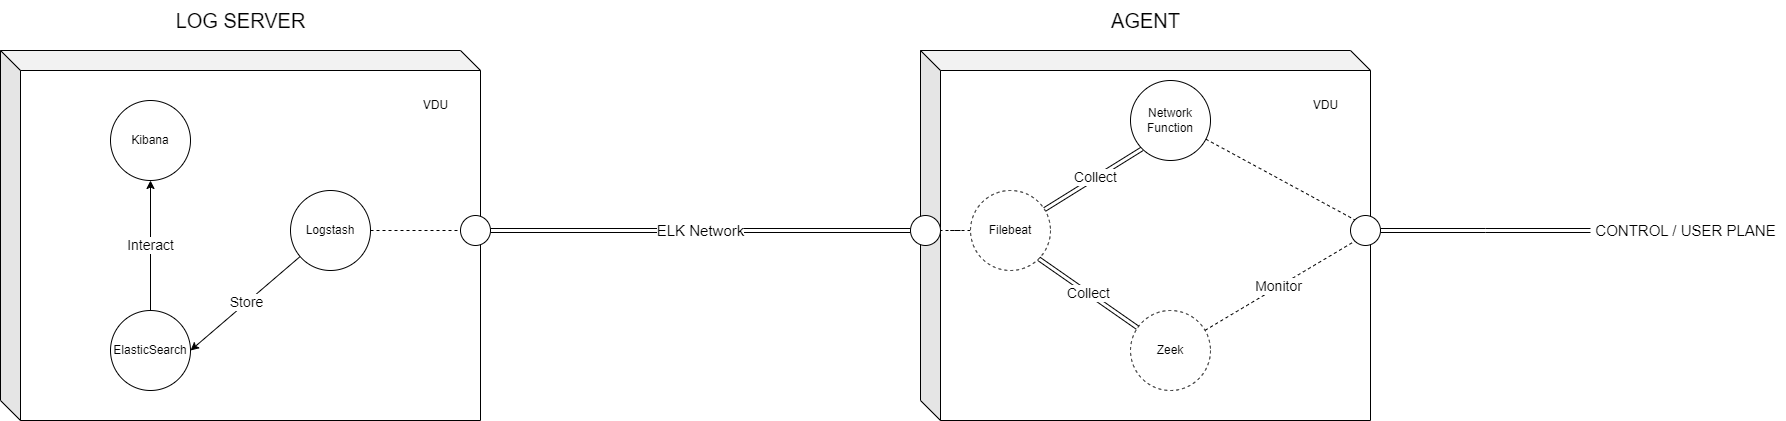
\includegraphics[width=1.15\textwidth, height=1.15\textheight, keepaspectratio]{diagrams/Basic_Prototype.png}
     \caption{5GDFRT Prototype}
     \label{fig:basic_prototype}
\end{figure}

Figure \ref{fig:basic_prototype} illustrates only one Log Server and Agent, however, you would typically have many agents all connected to one (or potentially many) log servers.

\subsection{Log Server - ELK Stack}
\label{sub3sub2}
The role of the Log Server is to securely ingest, store, manage, analyze, and visualize the collected log data. To facilitate this, we made use of the popular ELK stack. The ELK stack is a collection of three open-source projects, namely Elasticsearch, Logstash and Kibana.

\vspace{1em}

The ELK Stack is a centralized logging solution that is designed to manage and provide analytical tools for logs from distributed sources. Below, the role of each component is discussed in detail:
\subsubsection{Elasticsearch}
\label{sub3sub2sec1}
Elasticsearch is the core search and analytics engine in the ELK Stack and is based on  Apache Lucene \citep{bialecki2012apache}. Elasticsearch is a document-oriented database, a specific type of NoSQL database designed to store, retrieve, and manage documents, in this case, JSON documents. Which is perfect for handling the many different and varying types of logs that can be produced by network monitoring software. Elasticsearch stores and indexes all log data, making it easily searchable. Elasticsearch is also designed to be distributed with many nodes, providing high availability and data replication through data sharding. However, for the purposes of this project, we only utilized a single instance.
\subsubsection{Logstash}
\label{sub3sub2sec2}
Logstash is responsible for ingesting the data collected and forwarded by agents. Once received, it then transforms or filters the data if needed, and then forwards it to  Elasticsearch. Logstash can be used to preprocess and filter data such that data can be searched more effectively and efficiently. By offloading the preprocessing workload, Logstash helps minimize the processing burden on both the agents and Elasticsearch, enabling smoother and more scalable operation, especially in environments with high data throughput like 5G Networks. For this project, we utilized Logstash to create a pipeline that separates data collected by each agent into separate indices as well as adding fields that indicate when the data was received. This provides a useful mechanism to efficiently and effectively query data collected by each agent.
\subsubsection{Kibana}
\label{sub3sub2sec3}
The role of Kibana is to provide a user-friendly platform for interacting with the search and analytics engine (Elasticsearch). Kibana provides a web-based interface for visualizing and interacting with data. Key features include creating customizable dashboards and analyzing trends. Kibana also facilitates some of the more advanced features of Elasticsearch such as configuring machine learning tasks and setting up alerts. For this project, we utilized Kibana primarily for evaluation purposes and used many of the analytical features to search for patterns and create dashboards that capture trends.

\vspace{1em}

The ELK Stack (Elasticsearch, Logstash, and Kibana) is widely regarded as one of the most advanced and comprehensive centralized log collection and analysis solutions available today. In this section, we have only scratched the surface of its capabilities, which include powerful full-text search, real-time analytics, flexible data visualizations, advanced machine learning with anomaly detection, and many other features.

\vspace{1em}

The real benefit of the ELK stack is that it is designed for distributed environments. While, for this project, we only utilized a single Elasticsearch and Logstash instance, ELK can support multiple instances that are specialized for different tasks and can be scaled according to such tasks. This distributed approach could be leveraged to efficiently handle the high volume of information that may be collected from a complex 5G network.

\subsection{Agent}
\label{sub3sub3}
The Agent is responsible for monitoring, harvesting, and shipping potentially useful log data to support the storage and analysis of network events, including interactions between network functions and user traffic. Each Agent is installed on a Virtual Deployable Unit (VDU) hosting a network function and is configured to monitor both inbound and outbound traffic associated with that network function. The next few sections discuss the software components that make up the Agent.

\subsubsection{Zeek}
\label{sub3sub3sec1}
Zeek is an open-source software network analysis tool that is commonly used as a network security monitor (NSM) to support investigations of suspicious or malicious activity. In this case, Zeek is positioned to analyze and monitor traffic flowing through a network interface, specifically, the network interface utilized by the network function that it is monitoring. Zeek is capable of monitoring and capturing detailed information related to TCP/UDP/ICMP connections. It then stores this information in various detailed, highly structured JSON log files.

\vspace{1em}

Zeek produces many log files that capture multiple aspects of different types of traffic, however, the log files that were deemed most important are:

\begin{enumerate}[label=(\alph*)]
    \item \textbf{conn.log} \\
    Description: The conn.log or connection log is one of the more important logs produced by Zeek. It captures metadata from each observed connection, including originating/responding IP addresses and port numbers, timestamps, connection state, protocol (TCP, UDP, ICMP), duration, and the service involved (e.g., HTTP, SSL, DNS, other). This log is essential for understanding network behavior and is particularly useful for forensic analysis, incident response, and identifying anomalies in connection patterns. By analyzing the connection log, you can detect unauthorized access attempts, track the flow of data, understand the interactions between VNFs, and correlate events across different logs to establish a comprehensive picture of network activities.
    
    \item \textbf{http2.log} \\
    	Description: The HTTP/2 log captures metadata from HTTP/2 connections. Each log entry includes request/response headers, URI, URI parameters, and status codes. This log is one of the most useful logs, as 5G Core network functions that are 3GPP-Compliant communicate using HTTP/2. So by extracting the URI and URI values from HTTP/2 requests/responses, it can provide tremendous value with contextual information that can be used for event reconstruction.

    	
    \item \textbf{http.log} \\
    Description: The HTTP log collects metadata from HTTP/1.1 requests. As stated, 3GPP-Compliant network functions communicate using HTTP/2 or HTTP/3. However, collecting HTTP/1.1  logs can still be useful for non-standardized VNFs or perhaps providing more details on user traffic. Like http2.log, each log entry includes request/response headers, URI, URI parameters, and status codes.
    	
    \item \textbf{stats.log} \\
    Description: This log provides information regarding the performance of Zeek itself but is still useful, particularly for providing an overview of the current state of the network. Each log entry includes total packets processed/dropped, capture loss (packets that Zeek decided to, or could not process), and CPU/memory usage, total TCP/UDP/ICMP connections (alive/not). Unlike the other log types, the stats.log is generated at a configured frequency (every 300s). This log is particularly useful for detecting DoS attacks as it provides an overview of the total traffic that Zeek has processed within a specified period. So if there is a much larger than normal amount of packets being dropped we might be able to infer a DoS attack, by looking at the number of active connections for each traffic type we may even be able to conclude the type of DoS attack.
    
    \item \textbf{ssl.log} \\
    Description: The ssl.log captures detailed information related to SSL/TLS handshakes and connections. It can be used to help analysts understand encrypted communications, and detect possible malicious activity. Each entry corresponds to a specific SSL/TLS connection or handshake event and includes several important fields that describe the session including, timestamp, the origin/responder IP address, the cipher algorithm used, and the server name (e.g example.com).
    
    \item \textbf{dns.log} \\
    Description: The Domain Name System (DNS) log is one of the most important sources of data generated by Zeek. The log captures application-level name resolution activity. DNS logs can help identify suspicious or malicious domains that may be associated with malware, command and control servers, or phishing sites. By correlating DNS queries with other logs, investigators can piece together the timeline and nature of an incident, providing context for suspicious behavior. This log is particularly useful for analyzing user traffic. The information this log captures includes timestamp, origin/responder IP address, response code, and the query name.
    
    \item \textbf{notice.log} \\
    Description: This log captures alerts and notifications generated by Zeek when certain predefined conditions or patterns are met. This log is useful for highlighting potentially suspicious activities and security incidents that may require further investigation. Each entry typically includes information such as the timestamp, the origin/responder IP addresses, event type, and a description of the alert or message. This information can help forensic investigators to analyse security incidents effectively.
    
    \item \textbf{weird.log} \\
    Description: This log captures unusual or anomalous events that may not fit typical traffic patterns or behaviors. These unusual or anomalous events could indicate potential issues, misconfigurations, or even malicious activity. Each entry includes information such as the timestamp, the origin/responder IP addresses, a UID that references the connection, and a short description of the unusual behavior. The information can serve as a valuable resource for investigators looking to identify anomalies that may warrant further investigation.

\end{enumerate}

An important feature of Zeek is that it generates unique identifiers (UID) for each connection/event logged. This provides a useful mechanism for forensic investigators to analyze and correlate data across multiple different log entries and types. Effectively speeding up the forensic process, thus reducing cost. For example, a UID can be used to link HTTP requests in the http.log with its corresponding connection in the conn.log or perhaps a weird.log entry which is particularly useful. Each ID can serve as a reference point that links multiple log entries related to a single session or event recorded by a particular agent, which can aid in event reconstruction.

\vspace{1em}

The highly structured and well-labeled log data produced by Zeek enables more effective and efficient real-time analysis, offering capabilities that standard application logs generated by network functions typically cannot provide. Zeek’s logs are highly organized, with clearly defined fields for timestamps, source and destination IP addresses, protocol types, and unique identifiers for each network event. This structured format allows for effective parsing and indexing, making it possible to detect anomalies, track session flows, and identify suspicious patterns almost immediately as data is ingested. In contrast, application logs generated by network functions are often not standardized, lack uniformity and require additional complex preprocessing. Application logs also often require the context provided by surrounding log entries to be understood, making them even less reliable for real-time analysis. In comparison, Zeek logs provide consistent, self-contained details of each network event in a single log entry, making them far more reliable, actionable, and useful for effective real-time analysis.

\vspace{1em}

One of Zeek's most valuable features is its extensibility. It offers a powerful scripting language that enables developers to create custom rules and detection mechanisms. This customizability can be leveraged to meet specific needs and adapt to evolving network environments. A prime example of this extensibility is the HTTP/2 log. Although HTTP/2 is not supported by the base version of Zeek, a plugin called bro-http2, which uses the nghttp2 C library, extends Zeek's capabilities to monitor the more complex HTTP/2 traffic. This highlights how Zeek may be customized to add advanced features tailored to individual Virtual Network Functions (VNFs).

\vspace{1em}

Furthermore, this flexibility and customizability can be leveraged to address jurisdiction and regulatory compliance challenges mentioned in \ref{sub2sec3}. By configuring Zeek scripts for each agent, you can ensure that they comply with any applicable legal requirements. For example, in a highly distributed 5G Core Network with network functions deployed across different regions, Zeek scripts can be defined to align with the specific regulations of each region. This approach also extends to tools like Elasticsearch and Logstash, where different data retention, disclosure, and access policies may be set for each Log Server, ensuring that compliance is maintained across the entire system. This region-based configuration can be facilitated by Tacker's VNFD "flavors" by having a dedicated flavor for each network function for each region.

\subsubsection{Filebeat}
\label{sub3sub3sec2}
Filebeat is a lightweight, open-source data shipper that is part of the Beats family and is specifically designed for harvesting and forwarding log entries from log files. It integrates seamlessly with the Elastic Stack (ELK), making it a great choice for this DFR solution. Filebeat is responsible for securely harvesting, parsing, and hashing logs collected from both Zeek and the network function . Filebeat reads log files line by line and ships them to a designated output, however, it also allows for additional preprocessing steps. Recognizing the importance of data integrity in any DFR solution, we configured Filebeat to utilize a hashing function (SHA-256) that generates a digest based on the original log entry. This digest serves as a fingerprint of the log entry, allowing for later verification that the logs have not been tampered with. This mechanism for validation is crucial for forensic investigations, where the integrity and authenticity of the logs must be maintained. Filebeat was also configured to decode and parse the log entry into a format that is suitable for real time analysis.

\vspace{1em}

The ID and type of each VNF are also included in the log data to be transported. This will provide the necessary context for the documents and facilitate simple correlation during analysis, effectively speeding up an investigation. The basic structure of the final document shipped by Filebeat is shown in figure \ref{fig:document-structure}.
\begin{figure}[H]
    \centering
\begin{smalljson}
{
    "fields": {
      "digest": <DIGEST>, % Digest of original log entry
      "source": <LOG TYPE>, % Log source type (connection/dns/...)
      "vnf": <VNF_TYPE>, % Type of the VNF
      "id": <VNF_ID> % Unique ID for VNF instance
    },
    "input": {
      "type": "log" % Type of input
    },
    "agent": {
      "ephemeral_id": <AGENT_ID>, % Unique ID for agent
      "name": "filebeat", % Name of the agent
      "version": "8.15.0", % Version of the agent
      "type": "filebeat", % Type of the agent
      "id": <AGENT_ID> % Unique agent ID
    },
    "log": {
      "offset": 2500, % Offset in the log file
      "file": {
        "path": "path/to/log/file.log" % Path to the log file
      }
    },
    "message": "{...}", % Log entry (truncated)
    "@version": "1", % Version of the log format
    "@timestamp": "YYYY-MM-DDTHH:MM:SSZ", % Timestamp (When Filebeat processed it)
    "event": {
      "original": "{...}" % Original log entry (truncated)
    },
    "zeek/application": {
      "timestamp/ts": 1729950669 % Timestamp (When Zeek/NF generated the original log)      
      "field": "value" % Decoded/Parsed JSON field:value pairs
       ...
    },
    "host": {
      "name": <HOST_NAME> % Host name of the agent
    }
}
\end{smalljson}
\caption{Document Structure}
\label{fig:document-structure}
\end{figure}

\subsection{Data Flow}
\label{sub3sec3}

\begin{figure}[H]
  \centering
  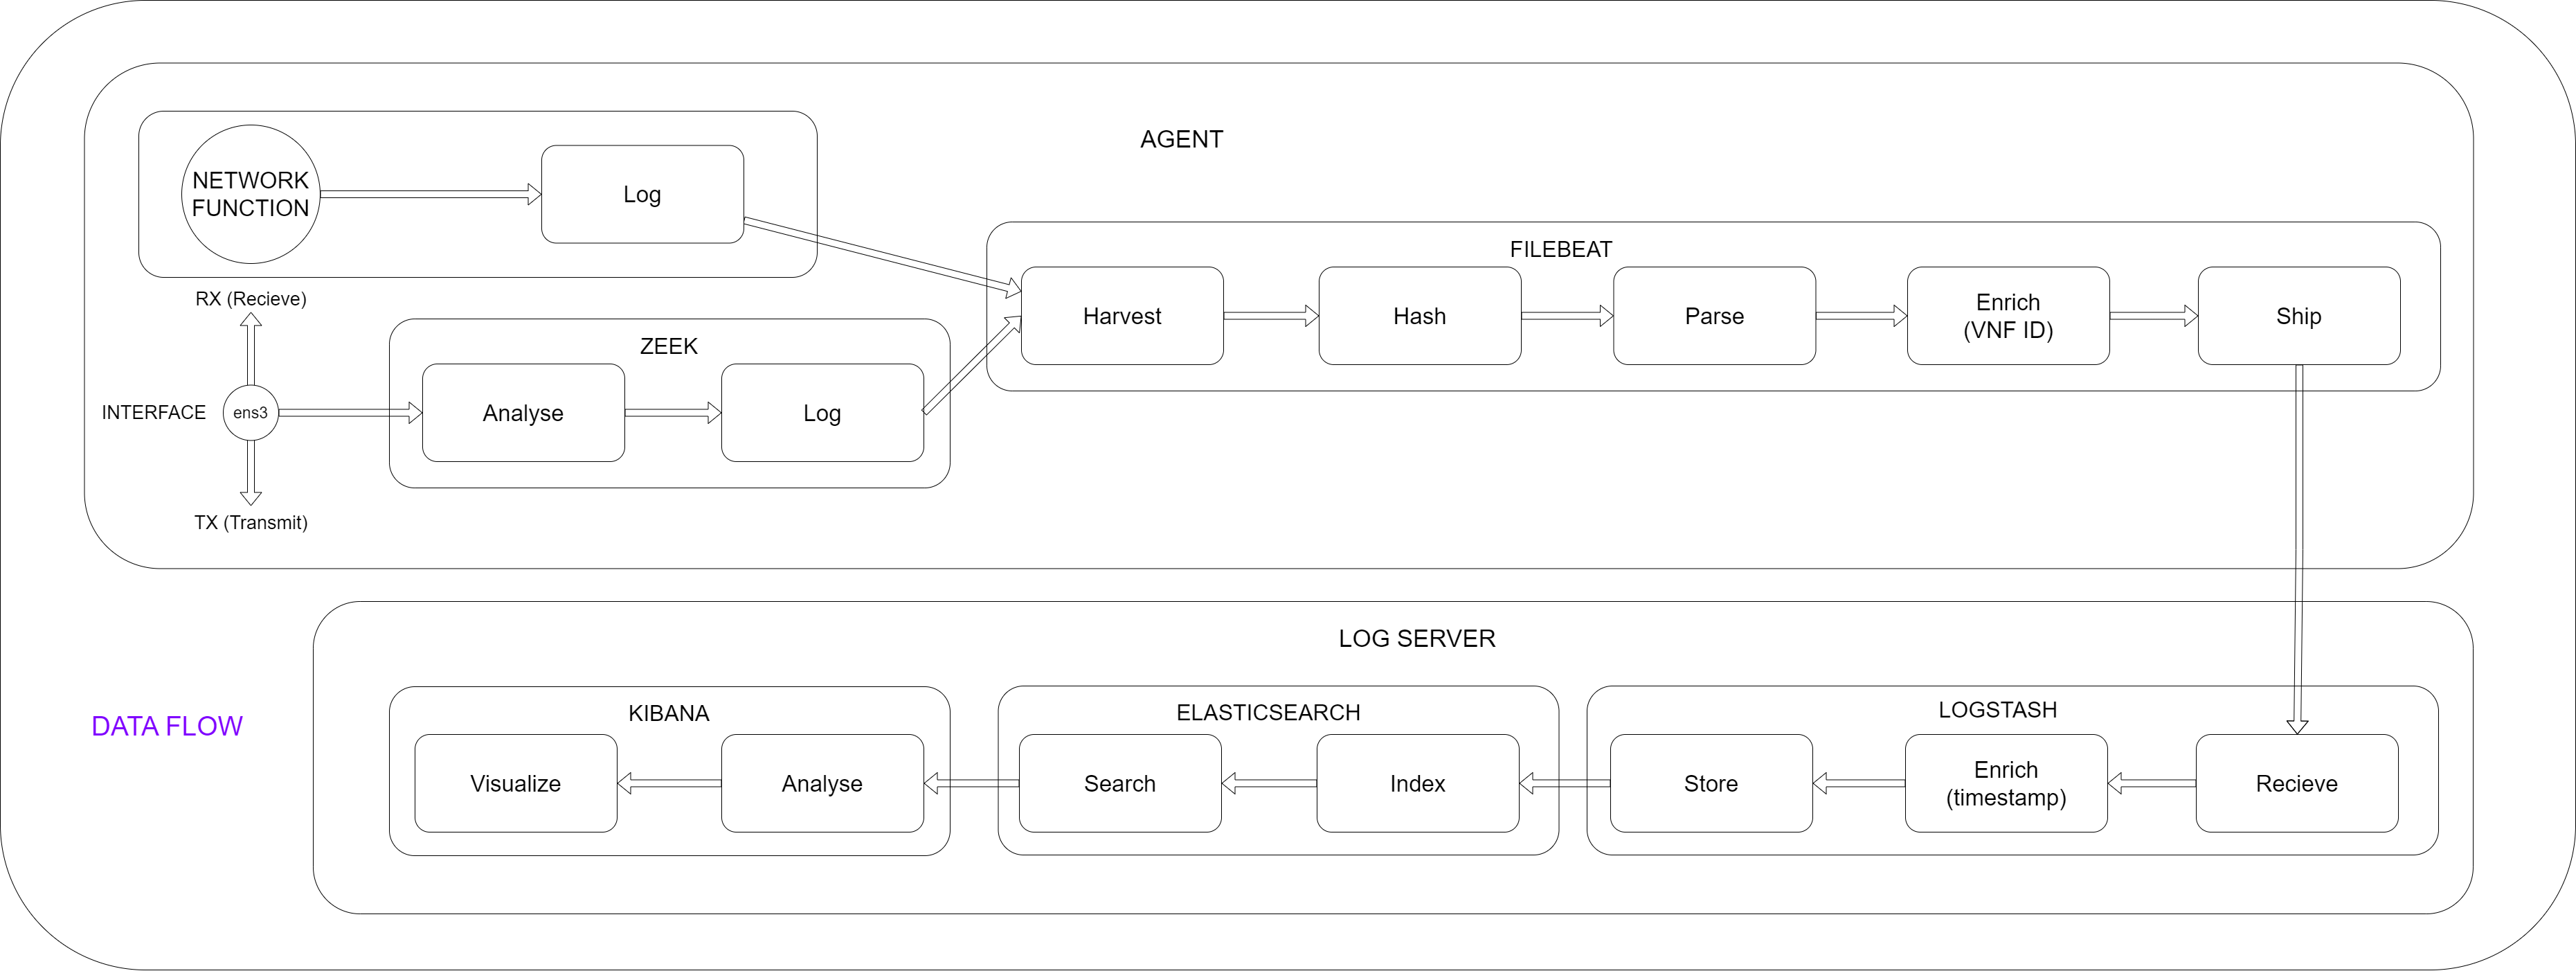
\includegraphics[width=\textwidth, height=\textheight, keepaspectratio]{diagrams/Flow.png}
  \caption{Log Data Flow}
  \label{fig:data-flow}
\end{figure}

Figure \ref{fig:data-flow} illustrates the basic flow of log data in the 5GDFRT. Firstly, the data is generated by Zeek or the network function, it is then harvested, hashed, decoded, and shipped by Filebeat. Next, it is received, timestamped, and sorted/stored by Logstash. Elasticsearch then indexes and facilitates analytical tasks. Finally, Kibana provides the mechanism to interact, analyze, and visualize the data. Some steps, such as authentication and encryption, discussed in the coming sections are not included in figure \ref{fig:data-flow} for brevity.

\subsection{Chain of Custody}
\label{sub3sec4}
The use of identifying information and timestamping shown in \ref{fig:document-structure} establishes a chain of custody for each document. This process includes several critical components:

\begin{itemize}
	\item "zeek.ts" and "zeek.uid": Indicate the original timestamp when the log was generated by Zeek and provide a unique identifier for the specific connection.
	\item "agent.id" (Filebeat agent ID) and "fields.id" (VNF ID): Identify which Virtual Network Function (VNF) and which Filebeat agent harvested and processed the log entry.
	\item "@timestamp": Marks the time when the log entry was processed by the Agent.
	\item "@received\_at": Records the time the log data was received and stored by Logstash. (Not shown in \ref{fig:document-structure})
\end{itemize}

The combination of these fields effectively forms a detailed history of the log data that documents its entire lifecycle, from its generation to its final storage. By linking each log entry to specific components, we can effectively establish a chain of custody, ensuring that the integrity and authenticity of the data can be verified and traced.

\subsection{Security}
\label{sub3sec5}
To meet both information assurance and possible regulatory requirements, multiple security features have been implemented that ensure Authentication, Access Control, Integrity, and Confidentiality of log data.

\subsubsection{Authentication and Access Control}
\label{sub3sub5sec1}
The ELK stack utilizes a Role-Based Access Control (RBAC) system to manage user credentials and permissions. For this project, we defined five users: logstash\_internal for Logstash, kibana\_system for Kibana, filebeat\_internal for Filebeat, and elastic (super-user) each with unique credentials required to authenticate access. This ensures that all incoming log data, from Agents, is coming from authenticated sources. It also ensures that all users (elastic) are also authenticated before they can access the log data.

\vspace{1em}

Additionally, two custom roles, logstash\_writer (assigned to logstash\_internal) and filebeat-writer (assigned to filebeat\_internal), grant specialized privileges, such as restricted write access to designated log data indices, an important aspect highlighted in \citep{tan2001forensic}. This ensures that filebeat\_internal (Filebeat) and logstash\_internal (Logstash) are the only users allowed to store log data in specific indexes. However, communication and the transfer of log data between Filebeat and Logstash uses a more advanced and secure Public Key Infrastructure (PKI) \citep{boldyreva2007closer} for authentication, ensuring a secure exchange with mutual certificate verification.

\subsubsection{Data in Transit - PKI}
\label{sub3sub5sec2}
As mentioned, Public Key Infrastructure (PKI) is used for authentication and communication between Filebeat and Logstash and ensures the security of data in transit between Filebeat and Logstash. PKI facilitates both mutual authentication between actors and the encryption of log data in transit. PKI utilizes asymmetric encryption to secure the data transmitted between Filebeat and Logstash. This is done by encrypting the log data with Logstash's public key, this way only Logstash can decrypt it using its private key. This prevents unauthorized actors from intercepting and reading sensitive log information during transmission, an important aspect of regulatory compliance (preventing PII disclosure). Using PKI allows for mutual authentication, where both Filebeat and Logstash verify each other's identities through the exchange of digitally signed certificates, ensuring that each party is communicating with a legitimate and trusted counterpart. This significantly mitigates the risk of man-in-the-middle attacks.

\subsubsection{Integrity - Hashing (SHA256)}
\label{sub3sub5sec3}
As mentioned, Filebeat uses a hashing function (SHA-256) to generate a digest of the original log entry before shipping it, along with various other identifying fields to Logstash. Hashing is an important part of any forensic investigation, as it provides a way to ensure that the logs remain immutable. Any modification to the log entry would result in a different hash value, alerting system administrators to potential tampering or data corruption, essentially assuring that the data has not been changed. This is particularly crucial in any forensic investigation, where maintaining the integrity of log data is essential for legal compliance and trustworthiness.

\subsection{Basic 5G Core Testbed}
\label{sub3sec6}
In this section, we will discuss the software, tools, and implementation details of the 5G Core Testbed used to evaluate our  5GDFRT. First, we discuss the software used for our 5G Core Network functions, followed by the details of the software used for simulating the Radio Access Network (RAN) and User Equipment (UE).

\subsubsection{5G Core Network - OAI}
\label{sub3sub6sec1}
For this project, we decided to use network functions developed by the Open Air Interface 5G (OAI-5G) Core Network (CN) project. The goal of the OAI-5G project is to provide 3GPP-Compliant 5G Standalone (SA) core network implementations that are both flexible and extensible.

\vspace{1em}

With OAI, the 5G Core is designed with a service-oriented architecture through the adoption of the new 3GPP defined SBA. In this architecture, a set of 5G Core NFs provide services to other NFs. For the interaction between network functions, one of these acts as a Service Consumer (Client), and the other as a Service Producer (Server).

\vspace{1em}

For our implementation of the 5G Core Network we decided to utilize a basic configuration with a single network slice and minimal resource requirements.

\begin{enumerate}
    \item \textbf{AMF:} The Access and Mobility Management Function (AMF)
    \item \textbf{SMF:} The Session Management Function (SMF)
    \item \textbf{UPF:} The User Plane Function (UPF)
    \item \textbf{NRF:} The Network Repository Function (NRF)
    \item \textbf{AUSF:} The Authentication Server Function (AUSF)
    \item \textbf{UDM:} Unified Data Management (UDM)
    \item \textbf{UDR:} Unified Data Repository (UDR)
\end{enumerate}

Each of these network functions handles a specific aspect of the 5G Core Network, and work together to handle UE registration and authentication (AMF, AUSF), PDU session management (AMF,SMF), network function discovery, user data storage and querying (UDM,UDR), policy enforcement (SMF), user traffic handling (UPF), along with many other functions.

\subsubsection{NF Intercommunication}
\label{sub3sub6sec2}
One important detail that should be highlighted is the manner in which Network Functions communicate and how we can capture this. As mentioned, in this architecture, network functions operate as client and/or server when interacting with one another. For this communication, network functions often utilize HTTP(S), HTTP/2, and HTTP/3 protocols, as defined by the 3GPP. OAI Network functions specifically utilize HTTP/2 to communicate.

\vspace{1em}

Capturing these interactions may provide useful information that can facilitate event reconstruction and by utilizing both Zeek (specifically the http2.log file) and the application logs, produced by the network function, we can effectively capture these interactions and events in great detail. Some of these events include:

\begin{itemize}
	\item Network Function Registration
	\item Data Access (UDR)
	\item UE Registration
	\item UE Authentication
	\item PDU Session Establishment/Modification/Termination
\end{itemize}

These are only a few of the events that we can capture and by securely collecting and storing this information, we should be able to effectively facilitate event reconstruction in the case of a security incident.

\subsubsection{RAN + UE Simulation}
\label{sub3sub6sec3}
As mentioned, the focus of this research is DFR in 5G Core Networks. However, to test and evaluate our 5GDFRT, we need to simulate RAN and UE interaction with the 5G Core Network. Therefore, we utilized three tools: UERANSIM, Ostinato, and SOCKS5 to simulate both RAN/UE interactions and to generate traffic.

\begin{figure}[H]
  \centering
  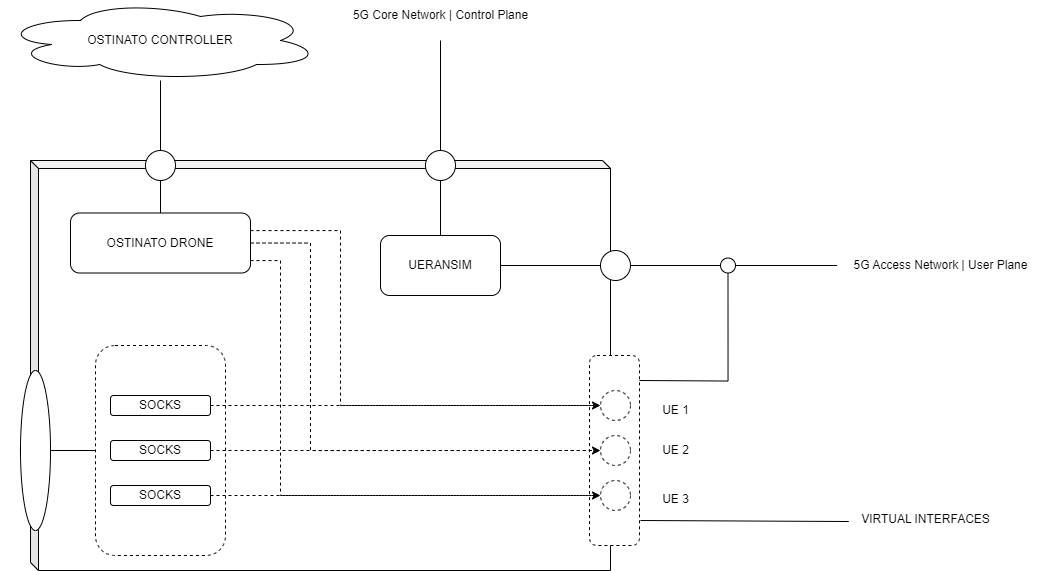
\includegraphics[width=\textwidth, height=\textheight, keepaspectratio]{diagrams/UERANSIM_Ostinato_SOCKS.png}
  \caption{Simulating the RAN}
  \label{fig:sim_ran}
\end{figure}

As illustrated in \ref{fig:sim_ran}, all these tools are hosted on a single VDU deployed via OpenStack through Tacker. The VDU is directly connected to the control and user plane through Neuron.

\paragraph{UERANSIM}
\label{sub3sub6sec3par1}
UERANSIM is an open-source, state-of-the-art 5G UE and RAN simulator. It implements 5G Standalone UEs and a 5G Standalone RAN. It simulates a 5G-enabled device and a gNodeB as a base station. UERANSIM uses configuration files for the gNodeB and each UE to register each of them with the 5G Core Network (AMF, AUSF). UERANSIM provides an interface for managing each UE that allows the establishment and management of PDU sessions. A PDU (Protocol Data Unit) session is essentially a logical connection between a UE (a user device) and the data network. In order to provide access to the 5G Core network using the PDU sessions, UERANSIM creates virtual interfaces, each of which is connected to the data network. These virtual interfaces serve as networking endpoints, effectively allowing our traffic generation tools to utilize a UE's PDU session.

\paragraph{Ostinato Drone + Controller}
\label{sub3sub6sec3par2}
Ostinato is a popular open source (up to version 1.3) traffic generation tool that can emulate and generate traffic for multiple devices using network interfaces, in this case, it uses the virtual interfaces created by UERANSIM to utilize a UE's PDU session. Ostinato provides detailed low-level control over the packets generated for each UE which allows us to generate many different types of traffic and control the amount and rate of packet generation. Ostinato is used extensively to evaluate our 5GDFRT prototype by generating many different types of malicious traffic. In Ostinato, multiple streams can be configured for each device. A stream is essentially a sequence of packets that you define and control for transmission over a network, it allows you to define the protocols used the number of packets transmitted, and the packet transmission rate. Ostinato also has a "Drone" feature that allowed us to control packet generation externally, simplifying the process.

\paragraph{SOCKS Proxy}
\label{sub3sub6sec3par3}
SOCKS5 Proxy server provides an additional method for traffic generation using externally hosted tools and applications. In this case, it was used in conjunction with Firefox and Python traffic generation libraries (Scapy) to generate typical browser traffic.

\subsection{DFR enabled 5G Core configuration}
\label{sub3sec7}
A final view of the 5G Core network is shown in figures \ref{fig:hl_config} and \ref{fig:ll_config}. Figure \ref{fig:hl_config} illustrates a simplistic view of the 5G Core Network configuration, indicating which network functions interact with each other. The area highlighted in green represents the network slice, with the UPF, SMF, and NRF. The user and control planes are indicated by the green and yellow lines respectively. The red is used to represent the interaction and transmission of logs between the Agents installed at each VNF and the ELK stack/Log Server. Figure \ref{fig:ll_config} illustrates a lower-level view of how the 5G Core Network, as defined in OpenStack. Here we can see that there are three separate Neuron networks: Control\_Network, N3\_Network, and the ELK network. Each Agent is connected to the Log Server (ELK stack) through the ELK network, and each VNF is connected to the 5G Control/N3 network. The figure also illustrates that Zeek is monitoring the interfaces utilized for the 5G Control/N3 networks.

\begin{figure}[H]
  \centering
  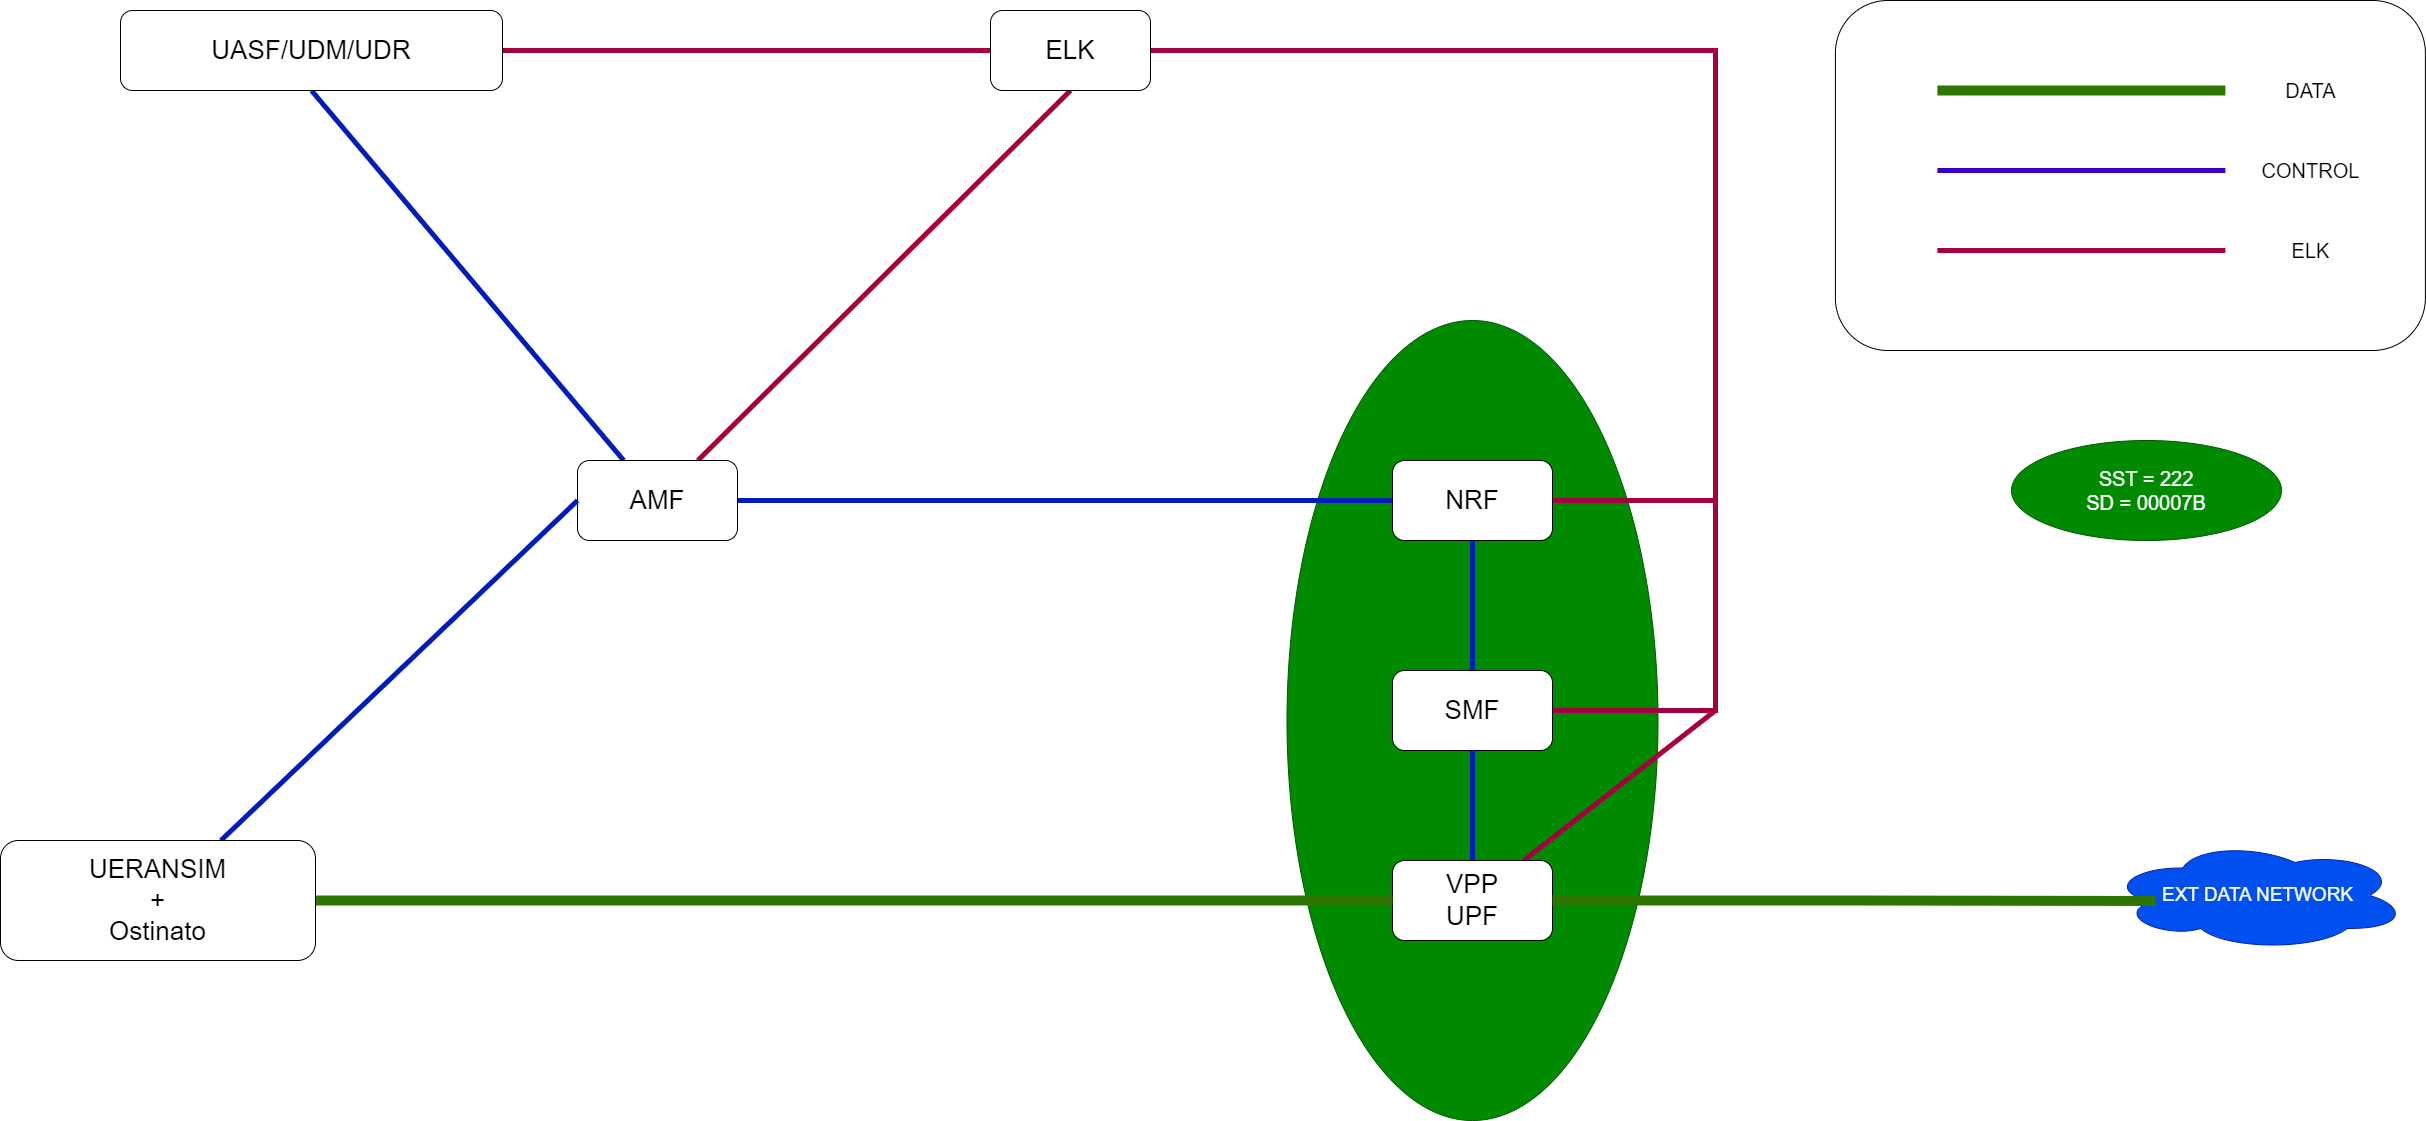
\includegraphics[width=\textwidth, height=\textheight, keepaspectratio]{diagrams/V6_Config_HL.png}
  \caption{High level view}
  \label{fig:hl_config}
\end{figure}
It is important to note the VDU marked EXT\_DN (External Data Network) in figure \ref{fig:ll_config}, this VDU essentially forwards traffic between the UPF and the external network using IP tables. This node also served as the target for our simulated attacks during experimentation and evaluation.
\begin{figure}[H]
  \centering
  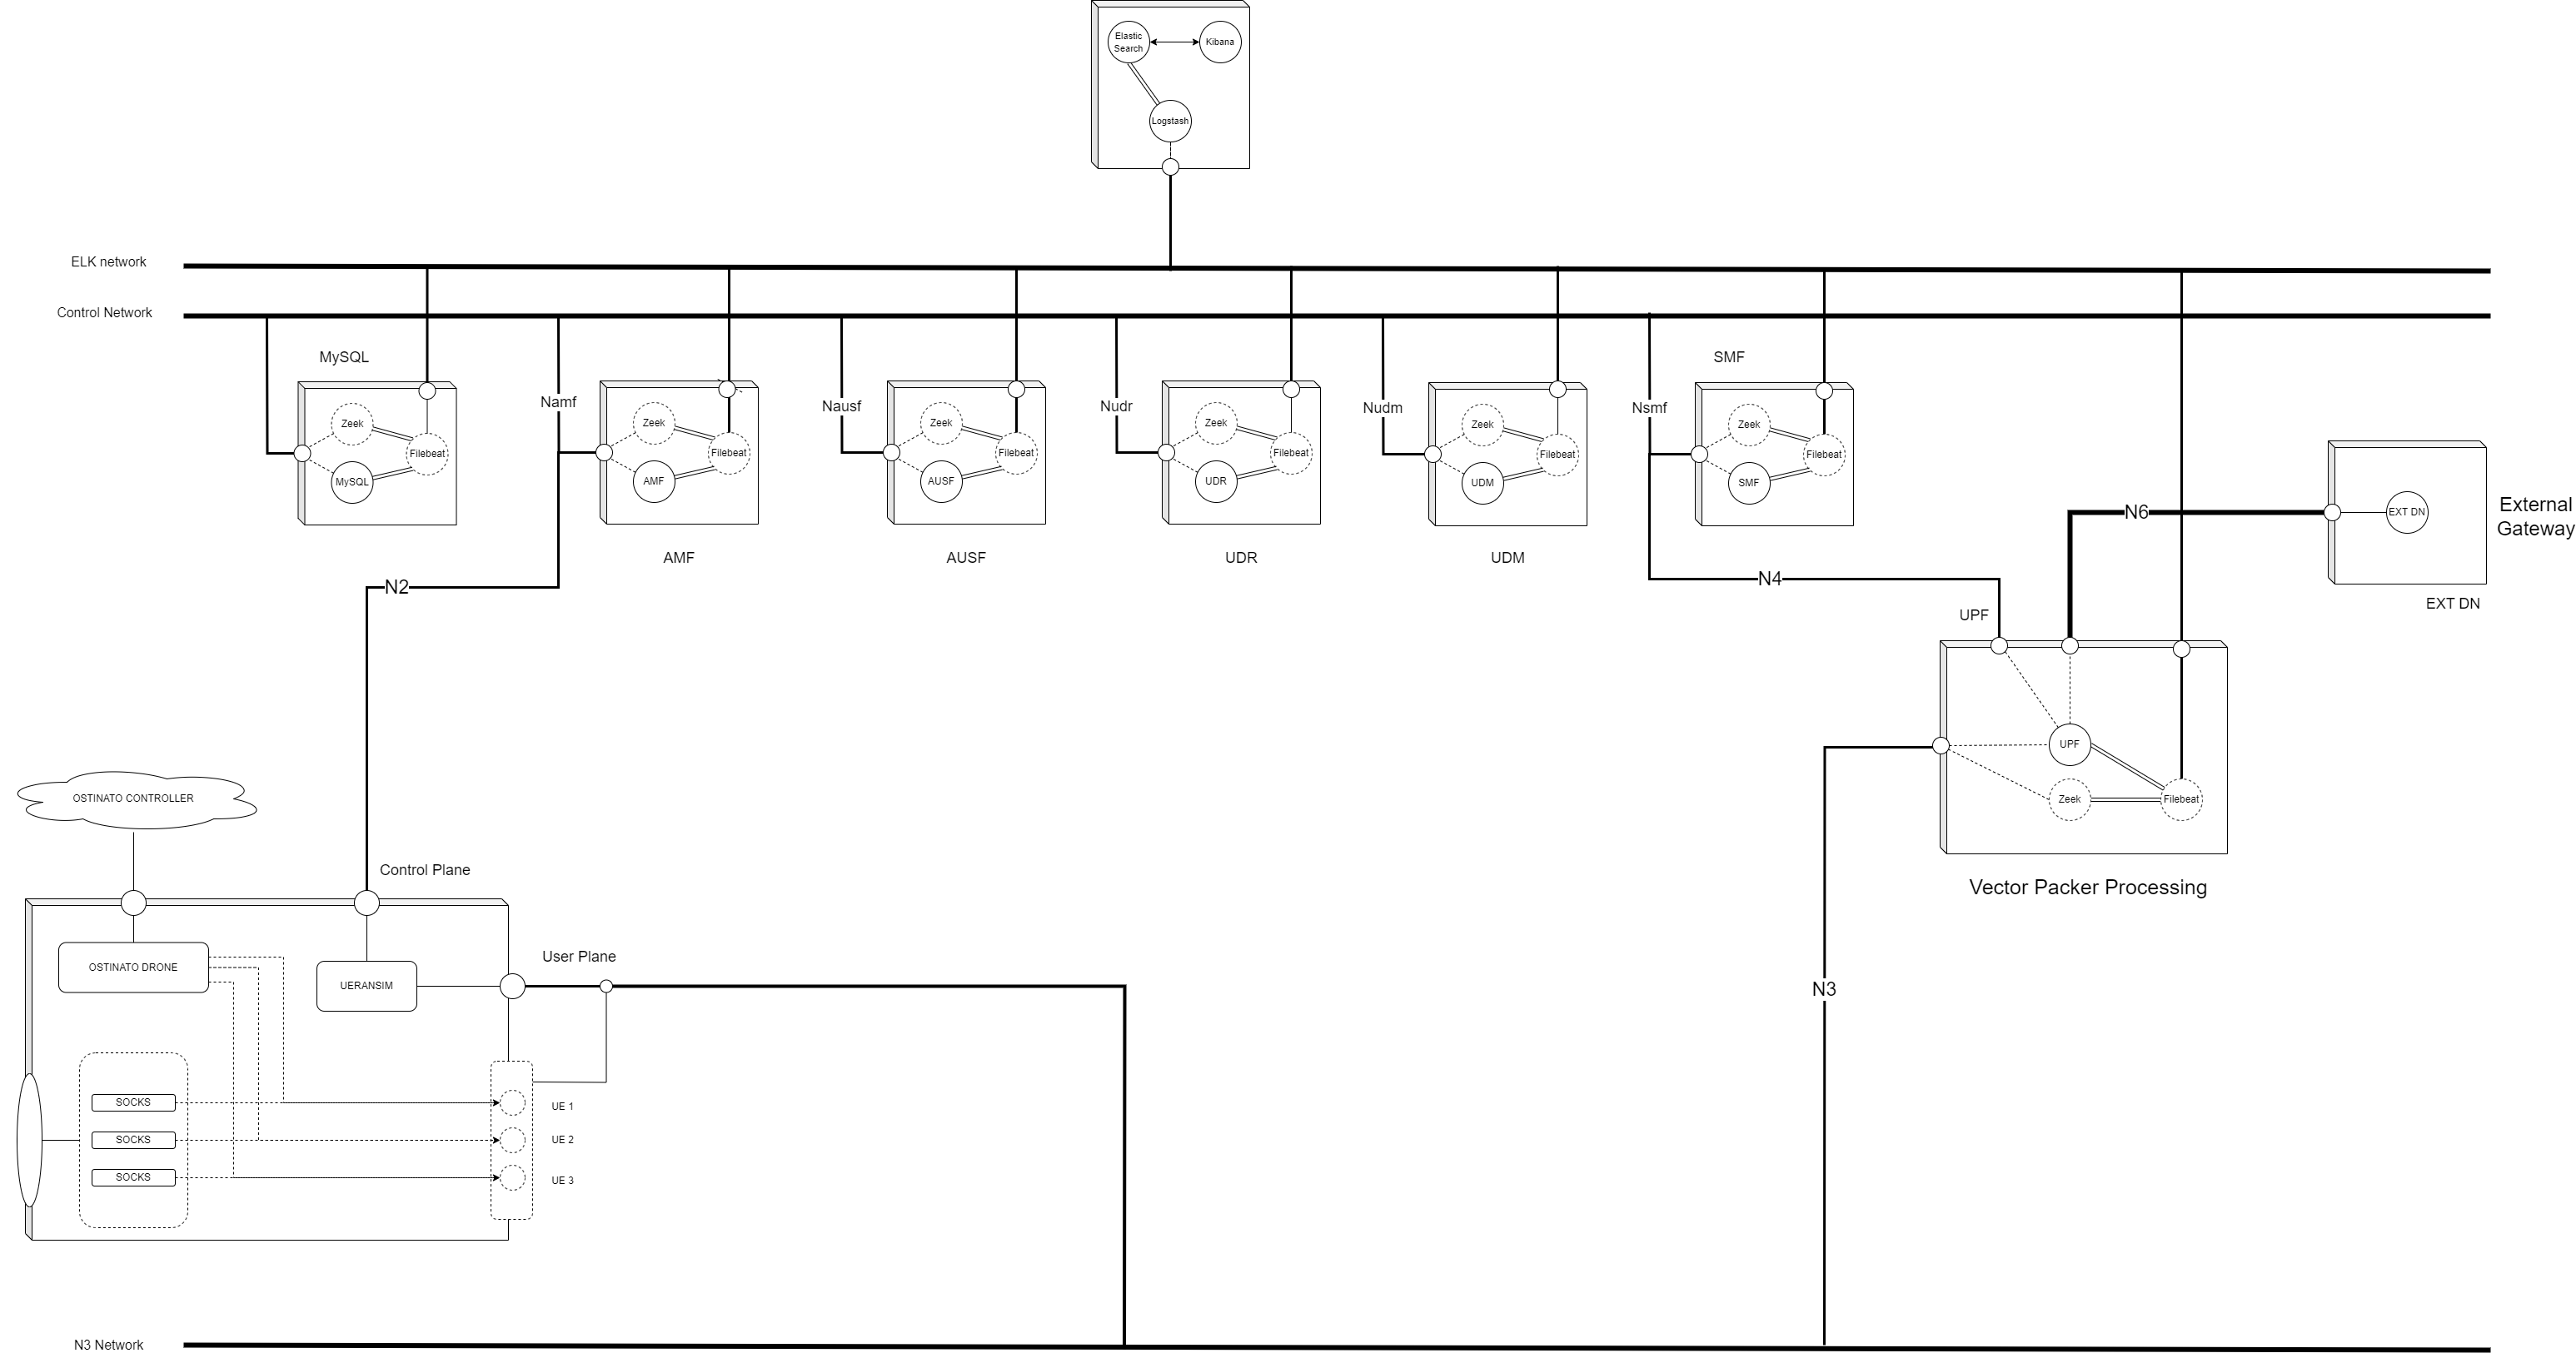
\includegraphics[angle=90, width=1.05\textwidth, height=1.05\textheight, keepaspectratio]{diagrams/Final_Config_LL.png}
  \caption{Low level view}
  \label{fig:ll_config}
\end{figure}
\newpage

\section{Prototype Experimentation and Insights}
\label{sec4}
In this section, we discuss the experiments that have been conducted to evaluate our 5G Digital Forensics Readiness Tool (5GDFRT). These experiments are rather simple but should provide the results needed to evaluate the 5GDFRT's ability to monitor our basic 5G Core Network. There are two main aspects in which the 5GDFRT needs to be evaluated. Firstly, there is its ability to detect malicious behavior in real time, and the second is event reconstruction. This section is constructed as follows, first, we discuss the experiments and results collected to evaluate real-time detection capabilities. Then, we discuss event reconstruction, with details related to NF communication and application logs.

\subsection{Real-time Detection}
\label{sub4sec1}
Two distinct scenarios were simulated using Ostinato. Each scenario models a common attack that the 5GDFRT should be able to detect and identify in near real-time. The target used for each attack is the EXT\_DN VDU referenced in figure  \ref{fig:ll_config}, it has been preconfigured with the IP address 10.7.0.4.

\subsection{DoS Ping Flood Attack}
\label{sub4sub1}
Denial of Service (DoS) attacks are a major issue for the networks of today and have been utilized to extort businesses and prevent access to legitimate users. DoS attacks overwhelm their target's resources and render them unavailable to legitimate users, which can have serious implications for the business operations of an organization. One such kind of attack is a Ping flooding attack. A Ping Flood Attack utilizes Internet Control Message Protocol (ICMP) echo requests to overwhelm the target. Each time the target receives the echo request, it will use a little computing power to process it and generate an ICMP echo reply. A Ping Flood Flood Attack takes advantage of this by generating tons of malicious ICMP echo requests, often from multiple devices (Distributed DoS), in order to overwhelm the target by consuming bandwidth and computing resources \citep{kumar2006ping}.\\

\subsubsection{Experimental Setup}
\label{sub4sub1sec1}
This Ping Flood Attack was simulated using Ostinato with 11 simulated UE devices. Figures \ref{fig:port-group} show the configurations used in Ostinato. It depicts the 11 virtual interfaces (uesimtunx) associated with each UE PDU session.

\begin{figure}[H]
  \centering
  \fbox{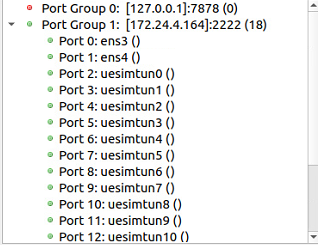
\includegraphics[width=0.6\textwidth, height=0.6\textheight, keepaspectratio]{images/Port_Group.png}}
  \caption{UE interfaces}
  \label{fig:port-group}
\end{figure}

A stream is configured for each interface (UE PDU session). The stream is configured to use 10.7.0.4 as the destination address and the source address is set to the corresponding PDU session IP allocated to each device. In the ICMP configuration, the ECHO request flag option is set, indicating that each packet is an echo request.

\begin{figure}[H]
  \centering
  \fbox{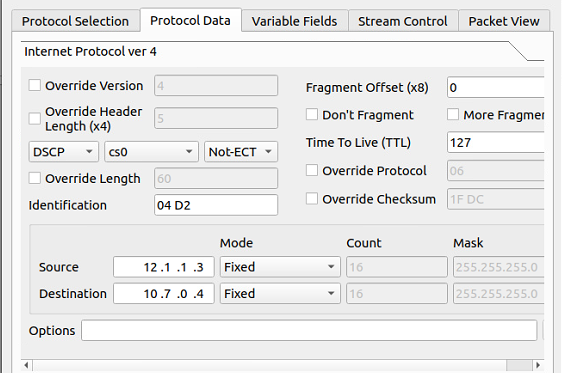
\includegraphics[width=0.6\textwidth, height=0.6\textheight, keepaspectratio]{images/ICMP_setup.png}}
  \caption{ICMP Setup}
  \label{fig:icmp-setup}
\end{figure}

Finally, the number of packets and the packet rate are set, using 1 Million packets at a packet rate of 2000 thousand packets per second. Meaning each device/stream would run for a total of 500 seconds.

\begin{figure}[H]
  \centering
  \fbox{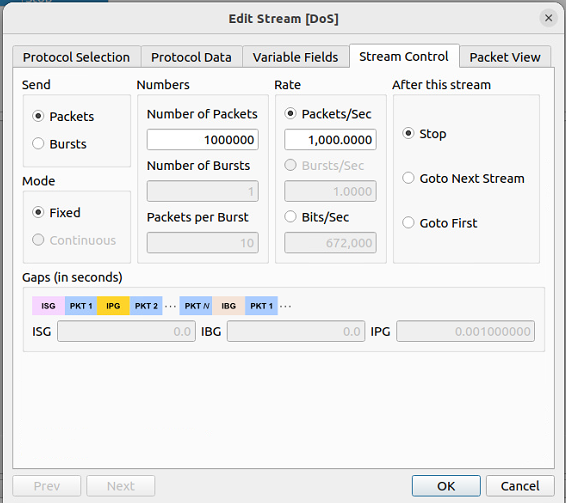
\includegraphics[width=0.6\textwidth, height=0.6\textheight, keepaspectratio]{images/Ostinato_Setup_2.png}}
  \caption{Packet Rate}
  \label{fig:port-group}
\end{figure}

\subsubsection{Results}
\label{sub4sub1sec2}
In order to best detect and visualize the collected log data we set up visualizations using Kibana. The best network function to analyze user-based attacks on other devices is the UPF function since it handles all user traffic in this configuration. However, if there are multiple network slices you would monitor each UPF allocated for each slice. For this visualization, we utilized the packets processed field of the stats.log produced by the Zeek.

\begin{figure}[H]
  \centering
  \fbox{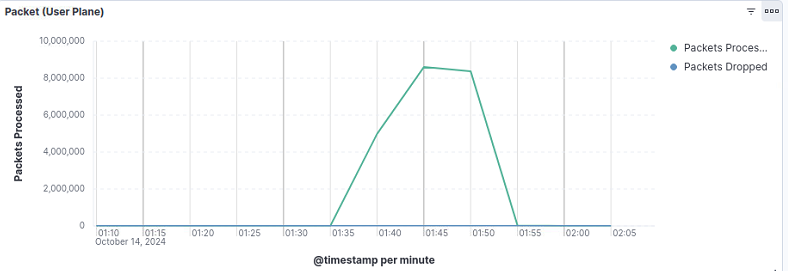
\includegraphics[width=\textwidth, height=\textheight, keepaspectratio]{images/DoS_Indication.png}}
  \caption{Packets Processed by UPF}
  \label{fig:dos-indication}
\end{figure}

As illustrated, in figure \ref{fig:dos-indication} the increase in traffic was clearly captured by the 5GDFRT, with almost 10 million packets being detected in the 300s intervals. You will notice a similar result by counting the number of ICMP connections generated in the conn.log. This same strategy can be applied to other types of DoS attacks such as UDP flooding, and TCP SYN flooding (the connection state of connections in the conn.log may further indicate this type of attack).
 
\subsection{IP Fragmentation Attack}
\label{sub4sub2}
The second attack scenario we simulated is an IP Fragmentation Attack. An IP fragmentation attack exploits how IP packets are fragmented and reassembled between devices. The attack involves manipulating offsets and sizes to trigger vulnerabilities of the victim/target host or even to evade security controls such as firewalls that would otherwise block traffic. IP fragmentation attacks avoid security controls by exploiting the fact that network devices and security systems often process each fragment independently without reassembling them for inspection, which can be used to avoid detection. They can also be used to exploit potential vulnerabilities in the target's IP packet processing mechanisms, potentially causing a crash, or some other undesired effect.

\subsubsection{Experimental Setup}
\label{sub4sub2sec1}
For this simulation we once again utilized Ostinato but, with a single UE device. We configured the stream to utilize a random offset value between 0 and 16 for each packet \ref{fig:frag-offset}, essentially overlapping and creating gaps between the received fragments, simulating the behaviour of an IP fragmentation attack.

\begin{figure}[H]
  \centering
  \fbox{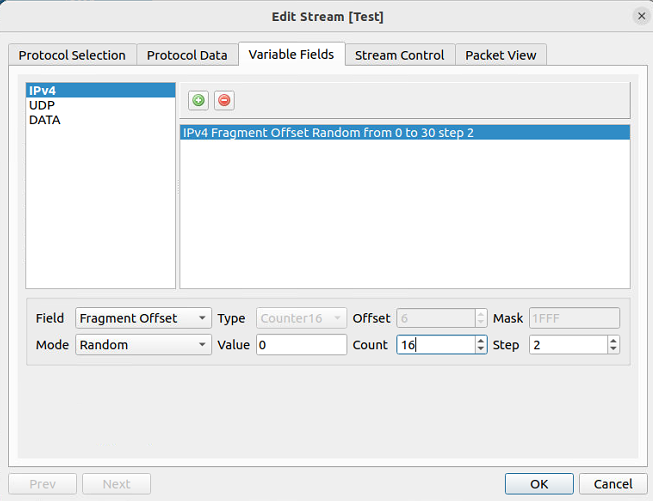
\includegraphics[width=\textwidth, height=\textheight, keepaspectratio]{images/Random_Frag_Offset_IP_FRAG.png}}
  \caption{Random Fragment offset}
  \label{fig:frag-offset}
\end{figure}

\subsubsection{Results}
\label{sub4sub2sec2}
Once again, we can detect this attack by looking at the log data collected by the Agent positioned at the UPF, specifically the weird.log data. As mentioned, the weird.log captures unusual and potentially malicious behavior. This includes overlapping and gaps in the fragment values of IP packets. This is illustrated in \ref{fig:ip-frag}, we can see that the weird log is reporting both fragment overlaps and fragment size inconsistencies. While this is not a definite indication that a fragmentation attack is occurring, if an unusual amount of such unusual behavior is present and continuous then it can be a definite indication that should require further investigation.

\begin{figure}[H]
  \centering
  \fbox{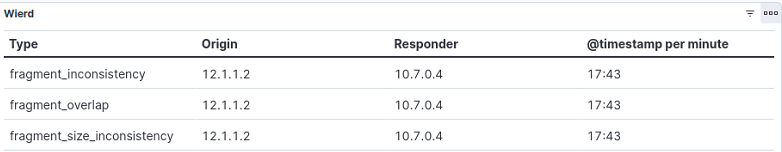
\includegraphics[width=\textwidth, height=\textheight, keepaspectratio]{images/viz_IP_FRAG.png}}
  \caption{IP Fragmentation alerts}
  \label{fig:ip-frag}
\end{figure}

\subsection{Event Reconstruction}
\label{sub4sec2}
As mentioned in \ref{sub2sub2sec1}, event reconstruction is one of the most vital processes in forensic investigations, and our 5GDFRT should be able to facilitate this. In 5G Core Networks, we can sort events into two main categories: Control Plane events, generated by interactions between network functions, and User Plane events, generated by user activity. Our 5GDFRT solution is able to capture both.

\subsubsection{Control Plane Events}
\label{sub4sub2sec1}
The Control Plane is responsible for managing signaling and orchestration between network functions, making Control Plane events a critical source of data for reconstructing events related to the state of the 5G Core Network. These Control Plane events we refer to are related to the interactions between these network functions. The most valuable sources of information for these events are the application and HTTP/2 logs (NF communication).

\vspace{1em}

The HTTP/2 log data captured and shown in \ref{fig:nrf-events} provides essential details for tracing NF interactions. This includes fields like the origin and responder IP addresses, URI, and timestamps, which collectively offer insights into the timing and nature of these interactions.

\begin{figure}[H]
  \centering
  \fbox{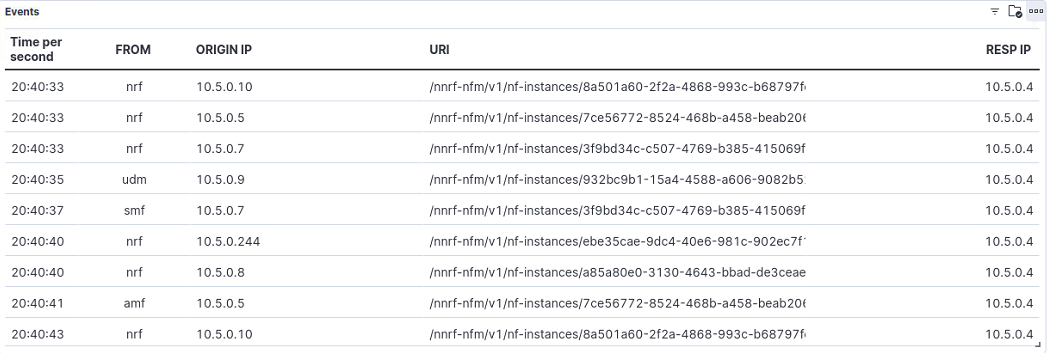
\includegraphics[width=\textwidth, height=\textheight, keepaspectratio]{images/EVENTS_NF_REGs.png}}
  \caption{NRF Events}
  \label{fig:nrf-events}
\end{figure}

When looking at the collected logs you may notice that all the entries have similar URI values and the same responder IP Address (10.5.0.4). This is because these are the heartbeat signals that each network function sends periodically to the NRF to indicate its current status. These heartbeat signals are particularly useful for event reconstruction, as they establish a clear active lifetime for each network function.

\vspace{1em}

However, if we filter these events out  as in Figures \ref{fig:non-nrf-events-1} and \ref{fig:non-nrf-events-2}, we notice some of the other important interactions between network functions.

\begin{figure}[H]
  \centering
  \fbox{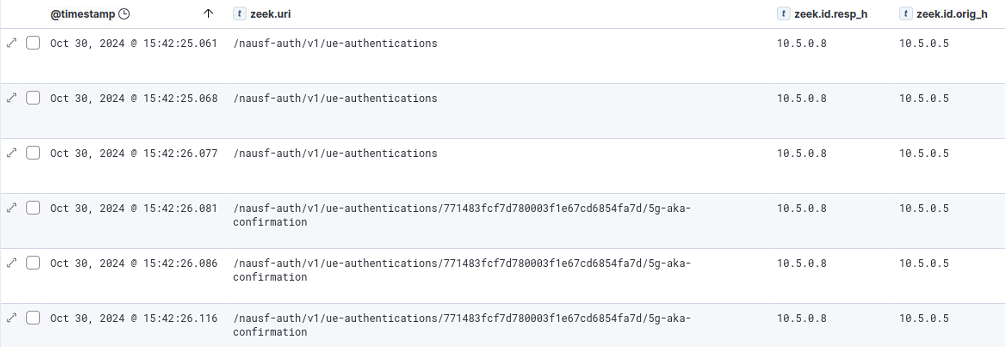
\includegraphics[width=\textwidth, height=\textheight, keepaspectratio]{images/HTTP2_log.png}}
  \caption{HTTP/2 Events 1}
  \label{fig:non-nrf-events-1}
\end{figure}

\begin{figure}[H]
  \centering
  \fbox{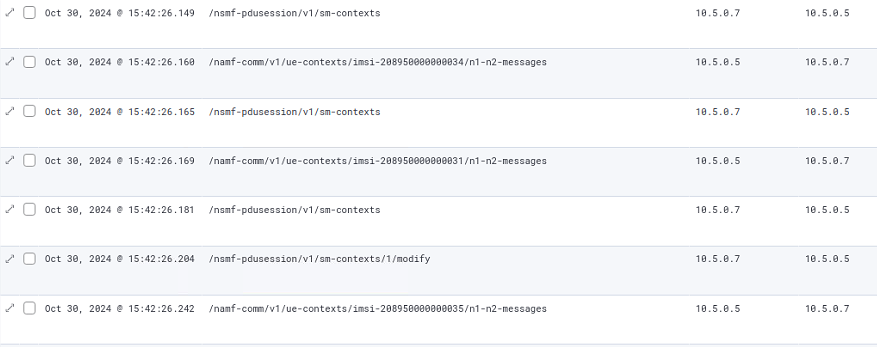
\includegraphics[width=\textwidth, height=\textheight, keepaspectratio]{images/HTTP2_Log_1.png}}
  \caption{HTTP/2 Events 2}
  \label{fig:non-nrf-events-2}
\end{figure}

In Figure \ref{fig:non-nrf-events-1}  we are able to observe the UE registration and authentication process in action, specifically for three UEs. Like the heartbeat signals, this information can provide an indication of the window in which each UE is active. We can also see the PDU session establishment and modification requests in figure \ref{fig:non-nrf-events-2}. This is useful for indicating the state of a UE's PDU session at a given point in time. What is even more interesting is the IMSI values depicted. IMSI values. IMSIs (International Mobile Subscriber Identifier) are unique IDs that identify mobile subscribers of networks by their SIM cards. These identifiers are particularly useful as they can be used to identify the specific user involved in these requests.

\vspace{1em}

The application logs collected also reflect these observed interactions. In figure \ref{fig:app-logs-1} we can see the NF heartbeat signal request being processed and sent to the NRF. These logs provide even more context and value as they indicate the exact status (REGISTERED) of a given network function (AMF) at a given point in time (2024-10-29 18:56:42). By using timestamps we can even cross-reference these interactions between the Zeek and application logs, a particularly useful aspect for event reconstruction.

\begin{figure}[H]
  \centering
  \fbox{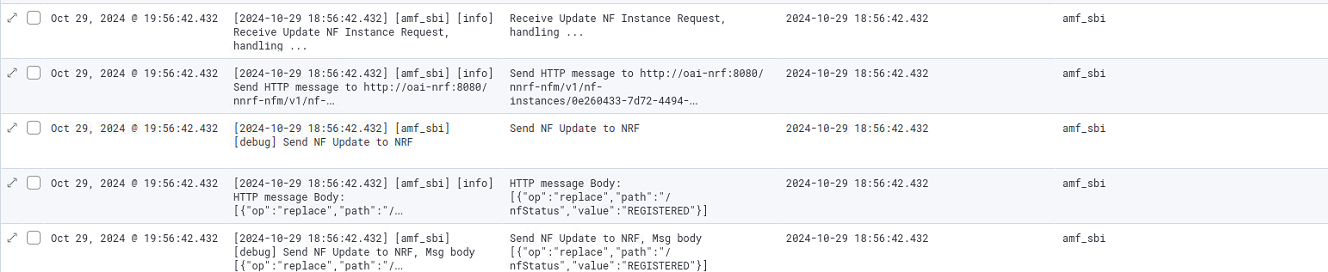
\includegraphics[width=\textwidth, height=\textheight, keepaspectratio]{images/Application_logs_0.png}}
  \caption{Application logs (AMF)}
  \label{fig:app-logs-1}
\end{figure}

The application log data collected from the AMF shown in \ref{fig:ue-device-table}, lists all active UE (User Equipment) devices along with their details, including the IMSI, NGAP ID, AMF UE ID, Cell ID, and PLMN (Public Land Mobile Network) ID. The PLMN ID contains both the MCC (Mobile Country Code) and MNC (Mobile Network Code) for each UE. This is quite clearly a valuable source of information and provides a comprehensive view of each active UE’s identity and location within the 5G core network. These attributes are highly valuable for event reconstruction, as they can be used by investigators to trace individual device activities and correlate network events. This level of detail is valuable in reconstructing the sequences of events related to UEs.

\begin{figure}[H]
  \centering
  \fbox{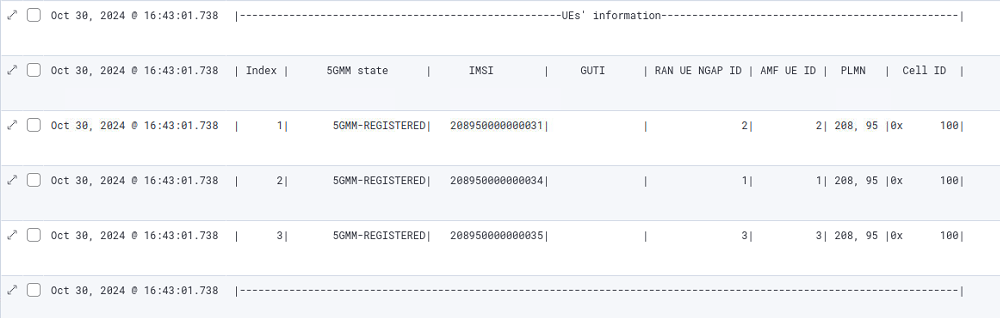
\includegraphics[width=\textwidth, height=\textheight, keepaspectratio]{images/UE_Device_Table.png}}
  \caption{UE Device Table (AMF)}
  \label{fig:ue-device-table}
\end{figure}

By combining the highly structured and well-labeled logs generated by Zeek with the detailed and valuable application logs collected from network functions, along with the identifying and timing information provided by our 5GDFRT \ref{fig:document-structure} \ref{fig:data-flow}, we are able to provide a comprehensive and accurate framework for event reconstruction. This integration ensures that all relevant data including network traffic behaviors, user activity related to function-specific interaction, and network function interactions in general are captured with precise timestamps and unique identifiers (Zeek UID, IMSI, IP) enabling an efficient and seamless platform for the reconstruction of events across the 5G Core network.

\subsubsection{User Plane Events}
\label{sub4sub2sec2}
The User Plane events we refer to are activities related to the user's interaction with the network, such as data transmission, browsing, or application usage. These events are generated based on the data traffic exchanged between the User Equipment (UE) and the network, typically involving interactions with external services, websites, or perhaps other users. As discussed earlier, this user traffic flows through the User Plane Function(s) (UPF). Therefore, by analyzing the log data generated by Zeek at the UPF(s), we can capture and examine these User Plane events.

\vspace{1em}

In order to test this we utilized the SOCKS5 proxy server, mentioned in 3.8.3.3, along with Firefox to generate browser traffic. It is important to note that the browser traffic was encrypted using HTTPS (a common situation), which meant that certain log types such as http.log and http2.log, which require unencrypted traffic, were not available. However, Zeek does provide a valuable log type specifically for this situation: the ssl.log. As mentioned in \ref{sub3sub3sec1}, this log captures information related to SSL/TLS sessions, allowing us to analyze secure communications and extract relevant data from encrypted traffic.

\vspace{1em}

We can observe this in the tabularized ssl.log data collected from the UPF in figure \ref{fig:ssl-browser-traffic}, with the origin and responder IP addresses and the specific service involved in the TLS handshake or TLS session.

\begin{figure}[H]
  \centering
  \fbox{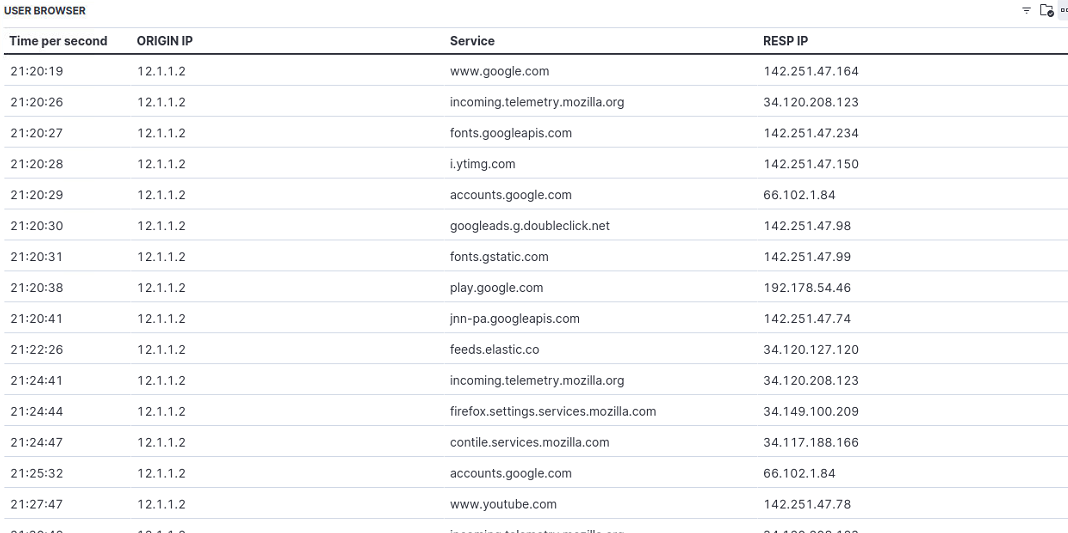
\includegraphics[width=\textwidth, height=\textheight, keepaspectratio]{images/SERVICE_USER_SSL.png}}
  \caption{Browser SSL log data}
  \label{fig:ssl-browser-traffic}
\end{figure}

Based on figure \ref{fig:ssl-browser-traffic}, we can see that the browser accessed different Google related services, including YouTube and Google fonts. It is clear that even for encrypted user traffic, the 5GDFRT solution was able to capture information that can aid in understanding what a user is doing at a given point in time. Furthermore, by combining and correlating this with the dns.log and conn.log data we can obtain an even greater understanding of a user's activities.

\newpage
\section{Evaluation}
\label{sec5}
In this section we focus on the analysis of our 5GDFRT and how it meets the requirements presented in \ref{sub2sub2sec1}. First we will start with monitoring, followed by information assurance, followed by cost and regulatory compliance. After that, we will discuss some of the issues and potential solutions to these issues. Finally, we will discuss some potential enhancements that could be included in a future implementation.

\subsection{Monitoring}
\label{sub5sec1}
As highlighted in Section 2.2 (Monitoring), the value of the data is crucial to DFR, and "What to log?" is an important question. For 5G Core Networks, it is clear that the data collected should be related to networking, traffic, and the state of VNFs. Zeek as a network security monitor combined with application logs proved to be perfect for this. Zeek managed to capture data that proved to be useful for both real-time detection and event reconstruction, while the application logs proved to be useful for capturing highly valuable and detailed information related to the state of both network functions and user devices, as illustrated in \ref{sec4}. Zeek's comprehensive logs allow analysts to easily correlate and identify unusual behavior effectively while the detailed application logs provided the missing application-level details and context that Zeek missed. And so by combining Zeek with application logs, we were able to collect and store useful data that facilitates a comprehensive and accurate framework for event reconstruction.

\subsection{Information Assurance}
\label{sub5sec2}
The use of ELK user credentials and roles effectively handles access control and authentication between Elasticsearch and the other components/users, while PKI addresses authentication and encryption between Logstash and Filebeat. Hashing ensured the integrity of the original log entry, while the final stored documents effectively captured the chain of custody from the point the log was generated, to when it was harvested and shipped until it was finally received and stored with information indicating exactly which components were involved. It is clear that the 5GDFRT effectively meets the Information assurance requirement.

\subsection{Cost and Regulatory Compliance}
\label{sub5sec3}
While both cost and regulatory compliance were considered out of scope for this project, the 5GDFRT was shown to have the capability to meet these requirements. With the lightweight and efficient nature of all the components involved, reducing costs and the extensibility and customisability of Zeek being able to operate under various regulations and performance requirements. While this does require further investigation, it is clear that a more comprehensive and abundant set of resources and expertise is required to effectively validate this.

\subsection{Issues}
\label{sub5sec4}
\subsubsection{Encrypted NF Communication}
\label{sub5sub4sec1}
While OAI 5G CN currently does not support TLS for communication between network functions, its implementation is a part of the 3GPP standard. While Zeek does offer some limited TLS 1.2 decryption capabilities (given the required key material), it is still not a supported feature. This degrades our ability to reconstruct events using HTTP/2 logs. That said Zeek is still able to collect useful information from both the ssl.log and the conn.log that are useful for capturing the interactions between network functions, however, they do not provide the same contextual value that the http2.log does.

\vspace{1em}

However, there are ways to handle this issue, such as the use of man-in-the-middle (MitM) proxies that handle decryption allowing Zeek to analyze the decrypted HTTP/2 traffic. This unfortunately introduces additional resource costs and latency that may not be acceptable for 5G Core Networks.

\vspace{1em}

Another approach demonstrated in \citep{wilkens2022passive}, shows that TLS decryption using Zeek is feasible without disrupting live communications. This approach leverages client-side integration to selectively forward TLS session key material to Zeek, allowing for passive decryption. While this avoids the complexity and latency of MitM proxies, it introduces additional operational challenges. One issue is that key material must be forwarded by clients very quickly to ensure full decryption. This would then require network function integration and additional processing which may not be acceptable.

\subsection{Potential Enhancements}
\label{sub5sec5}
\subsubsection{Application Integration}
\label{sub5sub5sec1}
While the logs generated by each network function do provide valuable information that can be used for event reconstruction, they do not provide the same detail and structure that allows for real-time detection and efficient analysis. This can be addressed if the 5G CN software is adapted to generate logs that are structured (JSON/XML), standardized, and rich in context. This in combination with the logs produced by Zeek would provide a more complete DFR solution.

\subsubsection{Specialization}
\label{sub5sub5sec2}
As mentioned in \ref{sub3sub3sec1}, Zeek provides a framework for creating customized scripts and configurations that can be applied based on the role and legal requirements of the network function it is monitoring. For example, the agent positioned to monitor the UPF may be under strict legal regulations that restrict the capture of certain types of user traffic. You can then configure Zeek to only capture information such as total packets processed/dropped and not HTTP or DNS requests. By specializing agents to comply with different legal requirements and VNF roles, we can effectively maximize the monitoring of the network while still complying with legal constraints.

\newpage
\section{Conclusion}
\label{sec6}
This research aimed to address the challenges of digital forensics introduced by the complexity and dynamic nature of 5G networks, as outlined in the problem statement. With 5G technology introducing significant advancements in telecommunications, such as increased scale, virtualization, and lower latency. These changes pose new obstacles to digital forensics and cybersecurity. As noted earlier, traditional forensic strategies are insufficient to address these challenges.

\vspace{1em}

In response to these challenges, we designed and implemented the 5G Digital Forensic Readiness Tool (5GDFRT), we then tested it using a basic 5G Core Testbed. The results demonstrated that the 5GDFRT was able to successfully detect common attacks, such as Denial of Service (DoS) and IP Fragmentation attacks, while facilitating secure log collection and event reconstruction. Although the prototype addressed key DFR requirements, further research is needed to assess its impact on 5G network performance and to tackle the cost and regulatory compliance challenges that will be crucial for real-world deployment.

\vspace{1em}

Ultimately, this work contributes to digital forensic readiness in 5G networks, providing a basic prototype and a broader proof of concept for how DFR strategies can be adapted to the unique characteristics of 5G. Further research will be needed to enhance the prototype and explore additional avenues, such as DFR in the Radio Access Network (RAN), as well as testing in more advanced 5G environments.

\newpage
\bibliographystyle{elsarticle-harv}
\bibliography{myBibFile}

\end{document}

\endinput